\ifdefined\included
\else
\documentclass[english,a4paper,11pt,twoside]{StyleThese}
\usepackage{amsmath,amssymb}             % AMS Math
\usepackage[T1]{fontenc}
\usepackage[utf8x]{inputenc}
\usepackage{babel}
\usepackage{datetime}

\usepackage{lmodern}
\usepackage{tabularx}
%\usepackage{tabular}
\usepackage{multirow}

\usepackage{subfigure}
\usepackage{fancyvrb}
\usepackage{algorithmic}
\usepackage{algorithm}
\usepackage{mathtools}


\usepackage{hhline}
\usepackage[left=1.5in,right=1.3in,top=1.1in,bottom=1.1in,includefoot,includehead,headheight=13.6pt]{geometry}
\renewcommand{\baselinestretch}{1.05}

% Table of contents for each chapter

\usepackage[nottoc, notlof, notlot]{tocbibind}
\usepackage{minitoc}
\setcounter{minitocdepth}{2}
\mtcindent=15pt
% Use \minitoc where to put a table of contents

\usepackage{aecompl}


% Glossary / list of abbreviations

\usepackage[intoc]{nomencl}
\iftoggle{ThesisInEnglish}{%
\renewcommand{\nomname}{Glossary}
}{ %
\renewcommand{\nomname}{Liste des Abréviations}
}

\newcommand{\accom}[1]{\textcolor{red}{[#1]}}

\makenomenclature

% My pdf code

\usepackage{ifpdf}

\ifpdf
  \usepackage[pdftex]{graphicx}
  \DeclareGraphicsExtensions{.jpg}
  \usepackage[a4paper,pagebackref,hyperindex=true]{hyperref}
  \usepackage{tikz}
  \usetikzlibrary{arrows,shapes,calc}
\else
  \usepackage{graphicx}
  \DeclareGraphicsExtensions{.ps,.eps}
  \usepackage[a4paper,dvipdfm,pagebackref,hyperindex=true]{hyperref}
\fi

\graphicspath{{.}{images/}}

%% nicer backref links. NOTE: The flag ThesisInEnglish is used to define the
% language in the back references. Read more about it in These.tex

\iftoggle{ThesisInEnglish}{%
\renewcommand*{\backref}[1]{}
\renewcommand*{\backrefalt}[4]{%
\ifcase #1 %
(Not cited.)%
\or
(Cited in page~#2.)%
\else
(Cited in pages~#2.)%
\fi}
\renewcommand*{\backrefsep}{, }
\renewcommand*{\backreftwosep}{ and~}
\renewcommand*{\backreflastsep}{ and~}
}{%
\renewcommand*{\backref}[1]{}
\renewcommand*{\backrefalt}[4]{%
\ifcase #1 %
(Non cité.)%
\or
(Cité en page~#2.)%
\else
(Cité en pages~#2.)%
\fi}
\renewcommand*{\backrefsep}{, }
\renewcommand*{\backreftwosep}{ et~}
\renewcommand*{\backreflastsep}{ et~}
}

% Links in pdf
\usepackage{color}
\definecolor{linkcol}{rgb}{0,0,0.4} 
\definecolor{citecol}{rgb}{0.5,0,0} 
\definecolor{linkcol}{rgb}{0,0,0} 
\definecolor{citecol}{rgb}{0,0,0}
% Change this to change the informations included in the pdf file

\hypersetup
{
bookmarksopen=true,
pdftitle="Joint Action for Human-Robot Interaction",
pdfauthor="Sandra DEVIN", %auteur du document
pdfsubject="Thesis", %sujet du document
%pdftoolbar=false, %barre d'outils non visible
pdfmenubar=true, %barre de menu visible
pdfhighlight=/O, %effet d'un clic sur un lien hypertexte
colorlinks=true, %couleurs sur les liens hypertextes
pdfpagemode=None, %aucun mode de page
pdfpagelayout=SinglePage, %ouverture en simple page
pdffitwindow=true, %pages ouvertes entierement dans toute la fenetre
linkcolor=linkcol, %couleur des liens hypertextes internes
citecolor=citecol, %couleur des liens pour les citations
urlcolor=linkcol %couleur des liens pour les url
}

% definitions.
% -------------------

\setcounter{secnumdepth}{3}
\setcounter{tocdepth}{2}

% Some useful commands and shortcut for maths:  partial derivative and stuff

\newcommand{\pd}[2]{\frac{\partial #1}{\partial #2}}
\def\abs{\operatorname{abs}}
\def\argmax{\operatornamewithlimits{arg\,max}}
\def\argmin{\operatornamewithlimits{arg\,min}}
\def\diag{\operatorname{Diag}}
\newcommand{\eqRef}[1]{(\ref{#1})}

\usepackage{rotating}                    % Sideways of figures & tables
%\usepackage{bibunits}
%\usepackage[sectionbib]{chapterbib}          % Cross-reference package (Natural BiB)
%\usepackage{natbib}                  % Put References at the end of each chapter
                                         % Do not put 'sectionbib' option here.
                                         % Sectionbib option in 'natbib' will do.
\usepackage{fancyhdr}                    % Fancy Header and Footer

% \usepackage{txfonts}                     % Public Times New Roman text & math font
  
%%% Fancy Header %%%%%%%%%%%%%%%%%%%%%%%%%%%%%%%%%%%%%%%%%%%%%%%%%%%%%%%%%%%%%%%%%%
% Fancy Header Style Options

\pagestyle{fancy}                       % Sets fancy header and footer
\fancyfoot{}                            % Delete current footer settings

%\renewcommand{\chaptermark}[1]{         % Lower Case Chapter marker style
%  \markboth{\chaptername\ \thechapter.\ #1}}{}} %

%\renewcommand{\sectionmark}[1]{         % Lower case Section marker style
%  \markright{\thesection.\ #1}}         %

\fancyhead[LE,RO]{\bfseries\thepage}    % Page number (boldface) in left on even
% pages and right on odd pages
\fancyhead[RE]{\bfseries\nouppercase{\leftmark}}      % Chapter in the right on even pages
\fancyhead[LO]{\bfseries\nouppercase{\rightmark}}     % Section in the left on odd pages

\let\headruleORIG\headrule
\renewcommand{\headrule}{\color{black} \headruleORIG}
\renewcommand{\headrulewidth}{1.0pt}
\usepackage{colortbl}
\arrayrulecolor{black}

\fancypagestyle{plain}{
  \fancyhead{}
  \fancyfoot{}
  \renewcommand{\headrulewidth}{0pt}
}

%\usepackage{MyAlgorithm}
%\usepackage[noend]{MyAlgorithmic}
\usepackage[ED=MITT - STICIA, Ets=INP]{tlsflyleaf}
%%% Clear Header %%%%%%%%%%%%%%%%%%%%%%%%%%%%%%%%%%%%%%%%%%%%%%%%%%%%%%%%%%%%%%%%%%
% Clear Header Style on the Last Empty Odd pages
\makeatletter

\def\cleardoublepage{\clearpage\if@twoside \ifodd\c@page\else%
  \hbox{}%
  \thispagestyle{empty}%              % Empty header styles
  \newpage%
  \if@twocolumn\hbox{}\newpage\fi\fi\fi}

\makeatother
 
%%%%%%%%%%%%%%%%%%%%%%%%%%%%%%%%%%%%%%%%%%%%%%%%%%%%%%%%%%%%%%%%%%%%%%%%%%%%%%% 
% Prints your review date and 'Draft Version' (From Josullvn, CS, CMU)
\newcommand{\reviewtimetoday}[2]{\special{!userdict begin
    /bop-hook{gsave 20 710 translate 45 rotate 0.8 setgray
      /Times-Roman findfont 12 scalefont setfont 0 0   moveto (#1) show
      0 -12 moveto (#2) show grestore}def end}}
% You can turn on or off this option.
% \reviewtimetoday{\today}{Draft Version}
%%%%%%%%%%%%%%%%%%%%%%%%%%%%%%%%%%%%%%%%%%%%%%%%%%%%%%%%%%%%%%%%%%%%%%%%%%%%%%% 

\newenvironment{maxime}[1]
{
\vspace*{0cm}
\hfill
\begin{minipage}{0.5\textwidth}%
%\rule[0.5ex]{\textwidth}{0.1mm}\\%
\hrulefill $\:$ {\bf #1}\\
%\vspace*{-0.25cm}
\it 
}%
{%

\hrulefill
\vspace*{0.5cm}%
\end{minipage}
}

\let\minitocORIG\minitoc
\renewcommand{\minitoc}{\minitocORIG \vspace{1.5em}}

\usepackage{multirow}
%\usepackage{slashbox}

\newenvironment{bulletList}%
{ \begin{list}%
	{$\bullet$}%
	{\setlength{\labelwidth}{25pt}%
	 \setlength{\leftmargin}{30pt}%
	 \setlength{\itemsep}{\parsep}}}%
{ \end{list} }

\newtheorem{definition}{Définition}
\renewcommand{\epsilon}{\varepsilon}

% centered page environment

\newenvironment{vcenterpage}
{\newpage\vspace*{\fill}\thispagestyle{empty}\renewcommand{\headrulewidth}{0pt}}
{\vspace*{\fill}}

\usepackage{tablefootnote}

\sloppy
\begin{document}
\setcounter{chapter}{0} %% Numéro du chapitre précédent ;)
\dominitoc
\faketableofcontents
\fi

\chapter{French extended abstract}

\label{ch:resume}

\selectlanguage{francais}
\section{Introduction}

Dans les années 40, des chercheurs inventent les premières machines appelées ordinateurs. En 1956, à la conférence de Darmouth, le domaine de l'intelligence artificielle est reconnu et les premiers robots arrivent rapidement dans notre environnement. Certains de ces robots vont devoir évoluer avec les Hommes ou dans leur entourage. Entre autres, les robots "co-workers" en industrie ou les robots sociaux \cite{dautenhahn2007socially}. Le but de cette thèse est de se rapprocher de robots qui peuvent agir conjointement avec les Hommes de manière naturelle, fluide et efficace. On se concentre ici sur les problématiques liées aux processus décisionnels durant l'action conjointe Homme-Robot. 

Dans un premier temps, basé sur une étude bibliographique des éléments nécessaires à l'action conjointe entre Hommes ainsi que sur des travaux existants en interaction Homme-Robot, les différents éléments nécessaires à l'action conjointe Homme-Robot seront identifiés ainsi que la manière dont ils peuvent s'articuler dans une architecture. Puis, l'architecture du superviseur, contribution technique principale de la thèse, sera présentée. Dans un second temps, mes travaux concernant l'amélioration de la gestion des plans partagés par le robot durant l'action conjointe seront présentés. La première amélioration concerne la prise en compte des états mentaux des Hommes durant l'exécution de plans partagés. La seconde contribution concerne le report de certaines décisions prises initialement par le robot durant l'élaboration du plan et à l'exécution afin d'obtenir une gestion plus flexible des plans partagés. L'évaluation de ces deux contributions en simulation et à l'aide d'une étude utilisateur sera également présentée. Finalement, dans un troisième temps, deux autres contributions à l'action conjointe Homme-Robot seront présentées. La première concerne la gestion du comportement non-verbal et plus précisément de la tête du robot. La seconde concerne l'association d'un système d'apprentissage à un système de planification dans le cadre de la prise de décision haut niveau.


\section{De l'action conjointe entre Hommes à la supervision pour l'interaction Homme-Robot}

\subsection{De l'action conjointe entre Hommes à l'action conjointe Homme-Robot}


\subsubsection{Théorie de l'action conjointe}

L'action conjointe a été décrite par \cite{sebanz2006joint} comme:

\begin{quote}
\textit{n'importe quelle forme d'interaction sociale où deux individus ou plus coordonnent leurs actions dans l'espace et le temps pour apporter un changement dans l'environnement.}
\end{quote}

Plusieurs prérequis sont nécessaires pour que deux individus réalisent avec succès une action conjointe. 

La première chose requise est que ces individus partagent un but et l'intention d'achever ce but. \cite{tomasello2005understanding} défini un but comme la représentation d'un état désiré par un agent et une intention comme un plan d'action qu'un agent s'engage à exécuter pour réaliser le but (basé sur le travail de Bratman \cite{bratman1989intention}). Dans le cas de l'action conjointe, une des définitions les plus reconnues est celle de Bratman \cite{bratman1993shared} qui présente trois conditions pour que deux individus partagent une \textit{intention jointe} d'accomplir un but G :
\begin{enumerate}
\item Chaque individu a l'intention d'accomplir G.
\item Chaque individu a cette intention en accord avec 1 et les parties du plan partagé de 1.
\item 1 et 2 sont une connaissance commune entre chaque individu.
\end{enumerate}
Cette définition est reprise et illustrée par Tomasello et al. dans \cite{tomasello2005understanding} (Fig.~\ref{fig:intention_jointe}). Ils définissent un \textit{but partagé} comme une représentation d'un état désiré plus la connaissance que le but va être réalisé en collaboration et une \textit{intention jointe} comme un plan partagé auquel les agents se sont engagés pour réaliser le but. Concernant ce plan partagé, cette notion a été introduite et formalisée par Grosz and Sidner \cite{grosz1988plans}. Leur définition suggère que chaque agent ne connaît pas nécessairement le plan entier mais seulement la partie qui le concerne et les parties en intersection avec celles de ses partenaires.

\begin{figure}[!h]
	\centering
    \includegraphics[width=\textwidth]{figs/Chapter1/intention_jointe.png}
    \caption{Exemple d'une activité collaborative par Tomasello et al. Ici les deux hommes ont pour \textbf{but partagé} d'ouvrir la boite ensemble. Ils ont choisi un moyen d'atteindre ce but qui prend en compte les capacités de chaque agent et ont donc une \textit{intention jointe}.}
    \label{fig:intention_jointe}
\end{figure}

Un deuxième prérequis de l'action jointe est que chaque agent doit être capable de percevoir et de prédire les actions de ses partenaires et leurs effets. A partir des travaux de \cite{sebanz2006joint}, \cite{pacherie2011phenomenology} et \cite{obhi2011moving} nous avons identifié plusieurs capacités nécessaires à ces prédictions :
\begin{itemize}
\item \textbf{L'attention jointe :} la capacité d'un agent à diriger son attention vers le même objet que ses partenaires de manière à partager la même représentation de l'environnement et des événements.
\item \textbf{Observation de l'action :} plusieurs études ont montré que quand quelqu'un observe une autre personne réaliser une action, une représentation de cette action est formée par l'observateur par ce qu'on appelle les \textit{neurones miroirs} et permet de prédire les effets de l'action \cite{rizzolatti2004mirror}.
\item \textbf{Co-représentation :} avoir une représentation de son partenaire (son but, ses capacités, ses connaissances, etc...) permet de prédire ses actions futures.
\item \textbf{Agency :} la capacité d'attribuer les effets d'une action au bon acteur.
\end{itemize}
Grâce à ces capacités, plusieurs prédictions peuvent être effectuées :
\begin{itemize}
\item \textbf{Quoi :} prédire quelle action un agent va réaliser.
\item \textbf{Quand :} prédire quand une action va avoir lieu et combien de temps elle va durer pour mieux se coordonner dans le temps.
\item \textbf{Où :} prédire les futures positions de ses partenaires pour mieux se coordonner dans l'espace.
\end{itemize}

Finalement, pendant l'action conjointe, les agents doivent être capables de coordonner leurs actions dans le temps et l'espace. Deux sortes de coordination sont définies dans \cite{knoblich20113} :
\begin{itemize}
\item \textbf{La coordination émergente :} qui a lieu intentionnellement. La coordination émergente peut être due à plusieurs mécanismes tels que \textit{l'entraînement} \cite{richardson2007rocking}, des \textit{affordances} communes \cite{gibson1977perceiving} ou la perception d'une action.
\item \textbf{La coordination planifiée :} qui est, elle, intentionnelle. Pour cela, les agents peuvent modifier leur comportement avec ce qui est défini par \cite{vesper2010minimal} comme des \textit{coordination smoothers} (mouvements plus prédictibles, signaux de coordination, etc...) ou utiliser la communication verbale ou non-verbale \cite{clark1996using}.
\end{itemize}


\subsubsection{Comment doter un robot des capacités nécessaires à l'action conjointe ?}

Plusieurs travaux ont déjà été réalisés afin de doter le robot des capacités nécessaires à la réalisation d'une action conjointe avec l'Homme. 

Dans un premier temps, le robot doit être capable de s'engager dans une action conjointe, de choisir un but. Ce but peut être imposé par l'utilisateur mais le robot doit aussi être capable de pro-activement proposer son aide. Pour faire cela, plusieurs travaux ont été réalisés concernant la reconnaissance de plans \cite{ramirez2009plan, bui2003general, singla2011abductive} et d'intentions \cite{breazeal2009embodied, baker2014modeling}. Le robot doit également être capable de choisir entre différents buts possibles. Pour faire cela le domaine de l'intelligence artificielle a commencé à proposer plusieurs solutions \cite{ghallab1994representation, lemai2004interleaving, roberts2016goal}. Une fois le robot engagé dans une action conjointe, il doit être capable de surveiller l'engagement de ses partenaires. Des réponses à ce problème ont été données en utilisant les signaux visuels et gestes \cite{sanghvi2011automatic} ou le contexte et les états mentaux \cite{salam2015multi}. Enfin, une fois le robot engagé dans un but, il doit être capable d'obtenir un plan partagé. Ce plan peut être imposé par l'utilisateur et le robot doit alors être capable de le comprendre \cite{pointeau2014successive, Mohseni2015} et éventuellement de le retransmettre \cite{petit2013coordinating, sorce2015proof}. Le plan peut aussi être construit en collaboration \cite{allen2002human} ou élaboré par le robot \cite{cirillo2010human,Lallement2014hatp}. Si le robot élabore le plan, il doit également être capable de communiquer à son sujet \cite{milliez2016using}.

Afin de mieux communiquer et travailler avec l'Homme, le robot doit être capable d'aligner sa représentation du monde (données en \textit{x, y, z} venant des capteurs) avec celle de l'Homme (relations sémantiques entre objets). Ce processus a été étudié et s’appelle \textit{l'ancrage} \cite{coradeschi2003introduction, mavridis2005grounded, lemaignan2012grounding}. Le robot doit également être capable de représenter son environnement non seulement de son point de vue mais aussi de celui de ses partenaires. La prise de perspective du robot \cite{breazeal2006using,milliez2014framework} peut être utilisée pour résoudre des situations ambiguës \cite{ros2010one}, mieux interagir durant le dialogue \cite{ferreira2015users} ou reconnaître et interpréter les actions de l'Homme \cite{baker2014modeling, nagai2015probabilistic}.

Finalement, le robot doit être capable de se coordonner avec l'Homme. A un haut niveau, l'Homme et le robot doivent coordonner leurs actions afin de réaliser le plan partagé avec succès. Plusieurs systèmes permettent de faire cela tels que \textit{Chaski} \cite{shah2011improved}, \textit{Pike} \cite{karpas2015robust} ou \textit{SHARY} \cite{clodic2009shary}. Pour faire cela, le robot doit se reposer sur ses capacités de communication verbale \cite{roy2000spoken, lucignano2013dialogue, ferreira2015users} et non-verbale \cite{breazeal2005effects, boucher2010facilitative, mutlu2009footing, hart2014gesture}. A un plus bas niveau, le robot doit se coordonner avec l'Homme durant l'exécution d'actions telles que le transfert d'un objet. Cela représente plusieurs challenges tels que trouver des postures acceptables par l'Homme \cite{cakmak2011human, dehais2011physiological, mainprice2012sharing}, approcher un Homme \cite{walters2007robotic} ou produire des trajectoires lisibles et prédictibles \cite{sisbot2012human, kruse2013human}.


\subsubsection{Une architecture trois niveaux}

Nous avons vu précédemment les prérequis pour l'action conjointe entre Hommes et Homme-Robot. Nous allons maintenant voir comment ces éléments se combinent en une architecture trois niveaux.

\begin{figure}[!h]
	\centering
    \includegraphics[width=0.8\textwidth]{figs/Chapter1/Pacherie.png}
    \caption{Les niveaux de Pacherie mis en cascade. Chaque niveau contrôle l'action à un niveau différent.}
    \label{fig:Pacherie}
\end{figure} 

En ce qui concerne l'action conjointe entre Hommes, Pacherie \cite{pacherie2011phenomenology} défend le fait que les processus liés à l'action conjointe se décomposent en trois niveaux qui ont chacun leur rôle  (Fig.~\ref{fig:Pacherie}) :
\begin{itemize}
\item \textbf{Shared Distal Intention :} c'est le niveau le plus haut. Ce niveau est responsable de la formation d'une \textit{intention jointe} et de la gestion du plan partagé.
\item \textbf{Shared Proximal Intention :} ce niveau a la responsabilité d'ancrer les actions reçues du niveau supérieur dans le contexte actuel. Cela doit être fait de manière coordonnée avec les partenaires de l'action conjointe.
\item \textbf{Coupled Motor Intention :} c'est le niveau le plus bas. Il est responsable des commandes moteurs des agents. Il s'occupe de la coordination spatio-temporelle au niveau le plus précis.
\end{itemize}

10 années avant que Pacherie développe ses idées concernant l'architecture trois niveaux, le domaine de la robotique autonome concevait intuitivement des architectures avec trois niveaux très similaires comme dans \cite{alami1998architecture} où l'on retrouve les niveaux :
\begin{itemize}
\item \textbf{Niveau décisionnel :} il est responsable de la production et la supervision du plan d'action. Il peut être comparé au niveau \textit{Distal} de Pacherie.
\item \textbf{Niveau exécutionnel :} il a la responsabilité de choisir, paramétrer et synchroniser les différentes fonctions nécessaires à l’exécution des actions venant du niveau décisionnel. Il peut être comparé au niveau \textit{Proximal} de Pacherie.
\item \textbf{Niveau fonctionnel :} il comprend toutes les foncions bas niveau d'action et de perception du robot. Il peut être comparé au niveau \textit{Motor} de Pacherie.
\end{itemize}

Cette architecture a été développée et adaptée au domaine de l'interaction Homme-robot. Récemment, nous avons présenté dans \cite{devin2016some} une version théorique d'une architecture adaptée à l'action conjointe Homme-robot (Fig.~\ref{fig:ArchiThreeLevels}).

\begin{figure}[!h]
	\centering
    \includegraphics[width=\textwidth]{figs/Chapter1/architecture.png}
    \caption{Architecture récente pour l'action conjointe Homme-robot. L'architecture est organisée autour des trois niveaux définis par Pacherie.}
    \label{fig:ArchiThreeLevels}
\end{figure}

\newpage
\subsection{Supervision pour l'interaction Homme-Robot}


\subsubsection{Rôle du superviseur dans l'architecture globale}

Le superviseur faisant l'objet de cette thèse fait partie d'une architecture globale pour l'interaction Homme-Robot développée au LAAS-CNRS. Une version simplifiée de cette architecture peut être trouvée Fig.~\ref{fig:GlobalArchi}. 


\begin{figure}[!h]
	\centering
    \includegraphics[width=0.7\textwidth]{figs/Chapter2/archiGlobal.png}
    \caption{Architecture globale pour l'interaction Homme-robot développée au LAAS-CNRS.}
    \label{fig:GlobalArchi}
\end{figure}

Cette architecture est composée de :
\begin{itemize}
\item \textbf{Un niveau sensorimoteur :} qui contient les modules bas niveau du robot lui permettant de gérer ses capteurs et actionneurs.
\item \textbf{TOASTER :} un module permettant au robot de représenter et maintenir un état du monde symbolique de son point de vue ainsi que de celui de ses partenaires.
\item \textbf{GTP :} un planificateur géométrique permettant au robot d'effectuer des actions en prenant en compte le confort et la sécurité de 
l'Homme.
\item \textbf{HATP :} un planificateur symbolique permettant au robot de calculer des plans pour lui même et pour ses partenaires afin d'atteindre un but donné.
\item \textbf{Un module de dialogue :} permettant au robot de communiquer avec l'Homme.
\item \textbf{Un superviseur :} ayant la charge de superviser l'activité du robot en coordonnant les autres modules. Il choisit le but du robot, veille au bon déroulement du plan partagé, choisit quand exécuter une action et comment communiquer.
\end{itemize}

L'architecture interne du superviseur peut être trouvée Fig.~\ref{fig:archiSup}. Il est composé de plusieurs modules :
\begin{itemize}
\item \textbf{Un gestionnaire de but :} permettant au robot de choisir quel but exécuter à chaque moment.
\item \textbf{Un élaborateur de plan :} permettant au superviseur de communiquer avec HATP afin d'obtenir un plan partagé.
\item \textbf{Un mainteneur de plan :} permettant au robot de suivre l'évolution du plan partagé.
\item \textbf{Un estimateur d'états mentaux :} permettant au robot d'estimer les états mentaux de ses partenaires humains concernant le plan partagé.
\item \textbf{Un module de décision :} permettant au robot de choisir quand exécuter une action ou donner une information.
\item \textbf{Un module d'exécution d'action :} permettant au superviseur de surveiller la bonne exécution des actions par le robot.
\item \textbf{Un module de communication non-verbale :} permettant de gérer pour le moment uniquement la tête du robot.
\end{itemize}

\begin{figure}[!h]
	\centering
    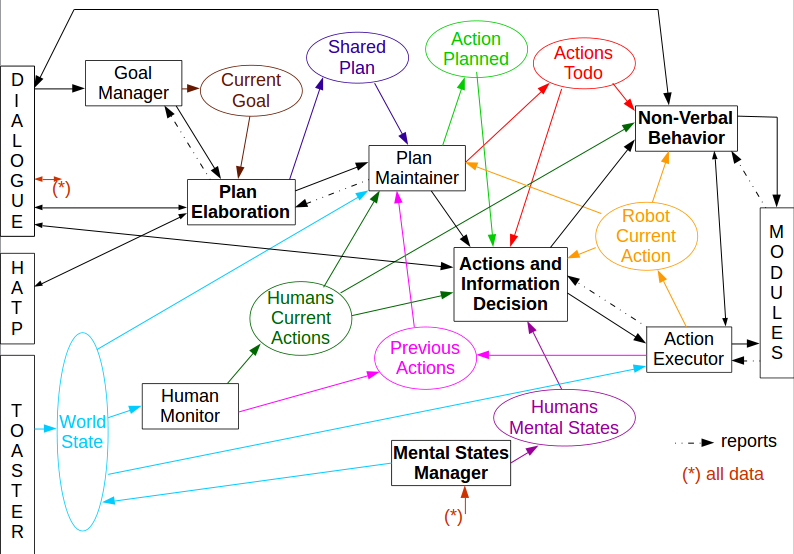
\includegraphics[width=\textwidth]{figs/Chapter2/ArchiSup.png}
    \caption{Architecture interne du superviseur. Les modules en gras sont traités dans ce manuscrit.}
    \label{fig:archiSup}
\end{figure}

\newpage
\section{Les plans partagés durant l'action conjointe Homme-Robot}

\subsection{Prendre en compte les états mentaux pendant l'exécution de plans partagés}

\subsubsection{Motivations et précédents travaux}

Quand le robot interagit avec un Homme, il est important qu'il ne le considère pas comme un outil ou un obstacle mais qu'il prenne en compte ses sentiments et son confort et donc son point de vue notamment lors de l'exécution d'un plan partagé.

La théorie de l'esprit désigne la capacité qu'ont les humains de reconnaître et s'attribuer des états mentaux en comprenant que les autres personnes peuvent avoir des connaissances et sentiments différents des leurs et de prendre en compte ces états mentaux pendant la prise de décision. La théorie de l'esprit a beaucoup été étudiée dans les sciences sociales \cite{baron1985does, premack1978does}, notamment la notion de prise de perspective qui désigne la capacité d'une personne à prendre le point du vue d'une autre personne \cite{tversky1999speakers, flavell1992perspectives}. Deux niveaux de prise de perspective sont définis dans \cite{flavell1977development}. La prise de perspective perceptuelle désigne la capacité d'une personne à comprendre que les autres ont une représentation du monde différente de la sienne (fig~\ref{subfig:conceptual}). La prise de perspective conceptuelle désigne la capacité d'une personne à attribuer des croyances et connaissances à une autre personne (fig~\ref{subfig:conceptual}).

\begin{figure*}[!h]
    \centering
    \subfigure[Prise de perspective perceptuelle: deux individus peuvent avoir deux représentations différentes de leur environnement.]{
        \centering
        \includegraphics[width=0.4\textwidth]{figs/Chapter3/perceptual.jpg}
       \label{subfig:perceptual}
   }\hfill
    %~
    \subfigure[Prise de perspective conceptuelle: ici Bob attribue à Alice une connaissance concernant la boite: il pense qu'Alice pense que la boite est vide.]{
        \centering
        \includegraphics[width=0.4\textwidth]{figs/Chapter3/conceptual.jpg}
       \label{subfig:conceptual}
    }
    \caption{Illustration de la prise de perspective perceptuelle et conceptuelle.}
\end{figure*}

En robotique, plusieurs travaux ont pour but de doter le robot de capacités liées à la théorie de l'esprit. Un des premiers travaux sur ce sujet est celui de Scassellati où il propose un modèle pour adapter deux modèles des sciences sociales \cite{leslie1984spatiotemporal, baron1997mindblindness} afin d'implémenter la théorie de l'esprit en robotique \cite{scassellati2002theory}. Plusieurs travaux ont permis aux robots de se doter de capacités de prise de perspective \cite{berlin2006perspective, hiatt2010cognitive, milliez2014framework}. Ces capacités ont été utilisées dans plusieurs travaux visant par exemple à mieux reconnaître et comprendre les actions de l'Homme \cite{johnson2005perceptual, baker2014modeling, nagai2015probabilistic} ou pour résoudre des situations ambiguës \cite{breazeal2006using}. Des travaux ont été réalisés pour prendre en compte le point de vue de l'homme durant l'élaboration d'un plan partagé \cite{warnier2012robot}, cependant, aucun ne concerne l'exécution de ce plan. Cette partie de la thèse a pour but de commencer à combler ce manque.

\subsubsection{Estimation des états mentaux}

Dans un premier temps le robot doit être capable d'étendre l'estimation des états mentaux de ses partenaires (qui concernait précédemment les connaissances sur l'environnement) aux connaissances concernant la tâche en cours et le plan partagé. Les algorithmes développés permettent au robot d'estimer les états mentaux de l'Homme concernant :
\begin{itemize}
\item \textbf{l'état du monde :} en plus de l'estimation des connaissances de l'Homme concernant l'état du monde observable venant de la prise de perspective (e.g. un objet est sur un autre objet) le robot est capable d'estimer les connaissances de l'Homme concernant l'état du monde non-observable (e.g. une boite est vide ou remplie) en se basant principalement sur les effets des actions.
\item \textbf{le plan partagé :} en se basant sur ce que l'Homme peut observer, le robot est capable d'estimer ses connaissances concernant les actions en cours ou passées. Grâce à cette estimation et à ses propres connaissances concernant le plan partagé, le robot est capable d'estimer les connaissances de l'Homme concernant l'état du plan (e.g. quelles actions doivent être exécutées).
\item \textbf{le but :} le robot est capable d'estimer des connaissances basiques de l'Homme concernant l'état du but en cours (e.g. si il est achevé) en se basant sur ses connaissances sur l'état du monde.
\end{itemize}

\subsubsection{Utilisation des états mentaux durant l'exécution du plan partagé}

Une fois les états mentaux de ses partenaires estimés, le robot doit être capable de correctement les utiliser afin de communiquer durant l'exécution du plan partagé quand une différence apparaît entre les connaissances du robot et celles de l'Homme. En effet, le robot doit fournir à l'Homme les informations dont il a besoin pour réaliser la tâche sans pour autant être trop verbeux en informant l'Homme à propos de tout et n'importe quoi. Pour cela, nous avons développé plusieurs comportements pour le robot :
\begin{itemize}
\item en accord avec la notion de \textit{weak achievement goal} de \cite{cohen1991teamwork}, si le robot détecte une différence entre ses connaissances concernant l'état du but en cours et celle d'un de ses partenaires, le robot va informer ce partenaire à propos de cette différence.
\item  lorsque le robot estime qu'un de ses partenaires doit effectuer une action, il vérifie si il estime que ce partenaire sait qu'il doit réaliser l'action. Si ce n'est pas le cas, le robot cherche la raison de cette différence de croyance et communique à ce propos.
\item lorsque le robot estime qu'un de ses partenaires pense qu'il doit effectuer une action, il vérifie si il estime également que l'action doit être réalisée. Si ce n'est pas le cas, le robot cherche la raison de cette différence de croyance et communique à ce propos.
\item quand le robot s’apprête à réaliser une action, il vérifie qu'il estime que ses partenaires sont au courant de cette action, et si ce n'est pas le cas, le robot signale son action avant d'agir.
\item finalement, comme l'estimation des connaissances de l'Homme par le robot peut être erronée, si le robot estime que l'Homme a toutes les connaissances pour réaliser une action mais que l'Homme n'agit pas, le robot va simplement demander à l'Homme de réaliser l'action et considérer que son estimation était erronée.
\end{itemize}

\subsubsection{Exemple illustratif}


\begin{figure}[!h]
	\centering
    \includegraphics[width=0.6\textwidth]{figs/Chapter3/cleanWithNames.png}
    \caption{État du monde au début de la tâche de nettoyage de table. Le robot peut atteindre le \textit{grey book} et le \textit{white book} tandis que l'homme peut atteindre le \textit{white book} et le \textit{blue book}.}
    \label{fig:initClean}
\end{figure}


Pour illustrer les bénéfices de ce travail, nous avons utilisé une tâche ou un Homme et un robot doivent nettoyer une table ensemble. Pour cela, ils doivent enlever tous les objets initialement placés sur une table (Fig.~\ref{fig:initClean}), puis le robot doit balayer la table et enfin les objets doivent être remis sur la table. Le plan initialement produit par le robot pour atteindre ce but est celui Fig.~\ref{fig:initPlanClean}.

\begin{figure}[!h]
	\centering
    \includegraphics[width=0.9\textwidth]{figs/Chapter3/InitCleanPlan.png}
    \caption{Plan initial pour la tâche de nettoyage de table.}
    \label{fig:initPlanClean}
\end{figure}

Le robot commence à enlever le \textit{grey book} pour le placer sur le meuble à côté de lui. Pendant ce temps, l'Homme enlève le \textit{blue book} et s'en va (Fig.~\ref{subfig:humanLeave}). Le robot termine son action. A ce stade du plan, la prochaine action qui doit être effectuée est celle de l'Homme (enlever le \textit{white book}). Comme l'homme ne revient pas, le robot calcule un nouveau plan où il enlève le \textit{white book} (Fig.~\ref{fig:newplan}).

\begin{figure}[!h]
	\centering
    \includegraphics[width=0.9\textwidth]{figs/Chapter3/SecondCleanPlan.png}
    \caption{Deuxième plan pour la tâche de nettoyage de table.}
    \label{fig:newplan}
\end{figure}

Le robot enlève le dernier livre et balaye la table (Fig.~\ref{subfig:robotSweep}). L'Homme revient alors (Fig.~\ref{subfig:humanComesBack}). Comme il peut voir que le \textit{grey book} est sur le meuble à côté du robot, le robot estime que l'Homme est capable de déduire par lui même que le robot a fini sa première action (enlever le \textit{grey book}). De même, comme l'homme peut voir le \textit{white book}, le robot estime également que l'homme est au courant que le robot a enlevé ce livre. Cependant, l'Homme ne peut pas observer que la table a été balayée (on considère ici que la table n'était pas très sale et que l'effet de balayer la table n'est pas observable). Comme l'Homme a besoin de savoir que la table a été nettoyée pour remettre le livre qu'il avait enlevé, le robot va l'informer à propos de cette action ("J'ai balayé la table."). L'Homme a donc toutes les informations nécessaires pour finir la tâche (et aucune information superflue qu'il pouvait observer de lui même), lui et le robot finissent donc la tâche avec succès (Fig.~\ref{subfig:endClean}).


\begin{figure*}[!h]
    \centering
    \subfigure[L'Homme part après avoir enlevé le premier livre.]{
        \centering
        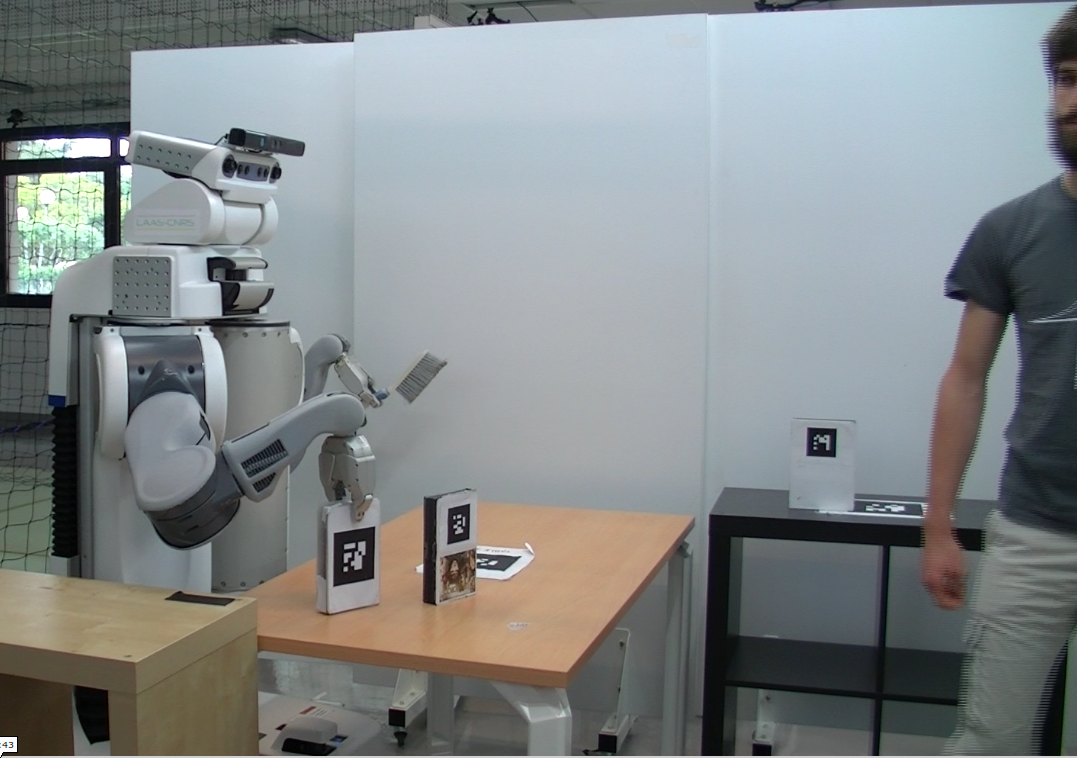
\includegraphics[width=0.4\textwidth]{figs/Chapter3/HumanLeave.png}
       \label{subfig:humanLeave}
   }\hfill
    %~
    \subfigure[Le robot enlève le dernier livre et balaye la table.]{
        \centering
        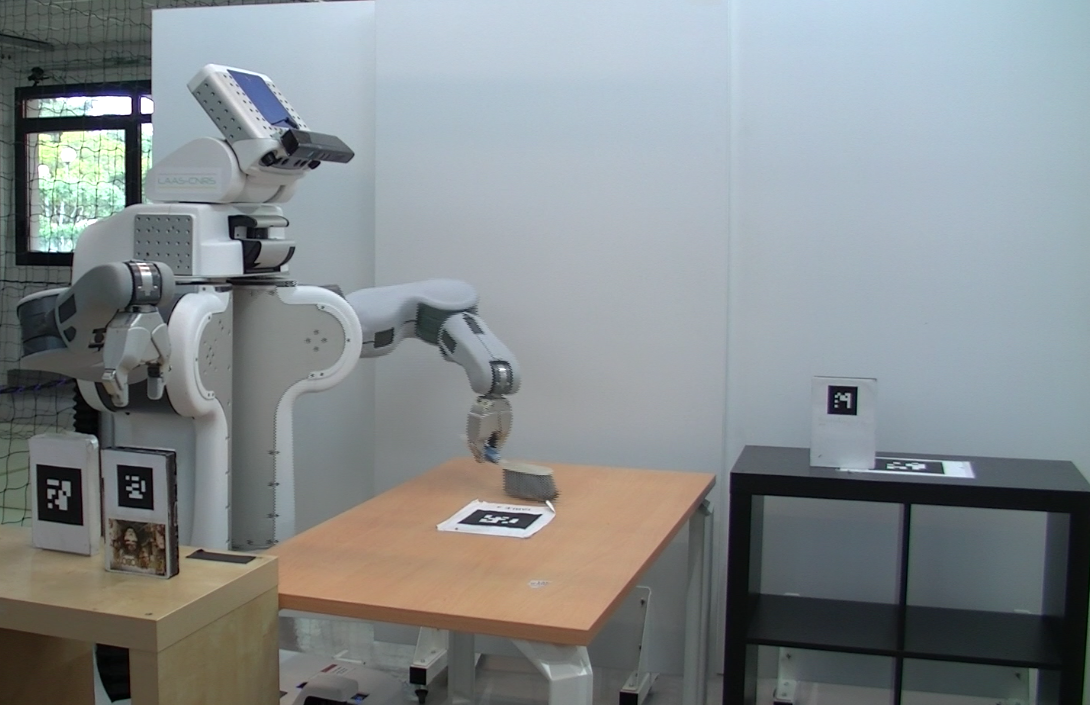
\includegraphics[width=0.44\textwidth]{figs/Chapter3/robotSweep.png}
       \label{subfig:robotSweep}
    }
    %~
    \subfigure[L'homme revient.]{
        \centering
        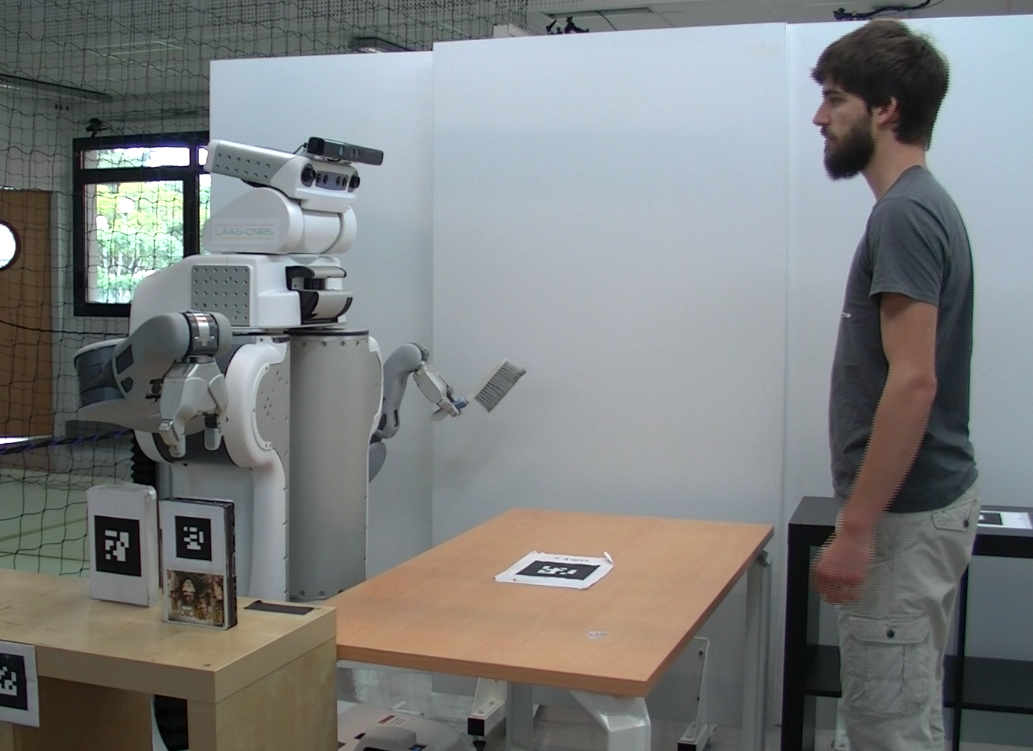
\includegraphics[width=0.4\textwidth]{figs/Chapter3/humanComesBack.png}
       \label{subfig:humanComesBack}
   }\hfill
    %~
    \subfigure[L'Homme et le robot finissent la tâche avec succès.]{
        \centering
        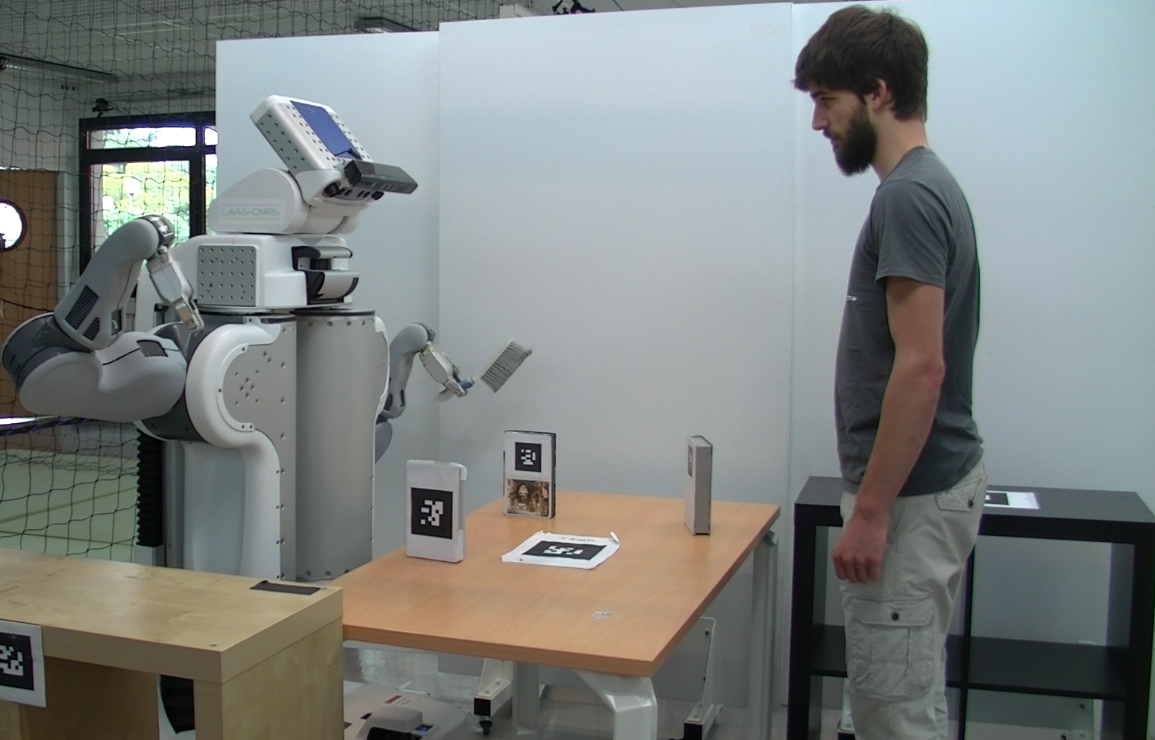
\includegraphics[width=0.45\textwidth]{figs/Chapter3/endClean.png}
       \label{subfig:endClean}
    }
    \caption{Exemple illustratif d'une tâche de nettoyage de table.}
\end{figure*}


\newpage
\subsection{Quand prendre les décisions pendant l'élaboration et l'exécution de plans partagés ?}


\subsubsection{Motivations}

Quand plusieurs individus collaborent lors d'une action conjointe, et plus particulièrement lors de l'exécution d'un plan partagé, de nombreuses décisions doivent être prises. Certaines d'entre elles vont être implicites alors que d'autres vont nécessiter une négociation ou une adaptation entre les acteurs de l'action conjointe. Afin d'être un bon partenaire, le robot doit donc être capable de prendre les bonnes décisions au bon moment et de correctement communiquer à leur propos (ne pas devenir trop verbeux en communiquant à propos des décisions implicites tout en donnant les informations nécessaires au bon déroulement de la tâche). Nous avons identifié trois types de décisions que le robot doit prendre durant l'élaboration et l'exécution d'un plan partagé :
\begin{itemize}
\item \textbf{Quelles actions exécuter dans quel ordre ?} cela a été le sujet de plusieurs travaux dans le domaine de l'interaction Homme-Robot. Nous utiliserons pour gérer ce type de décisions, HATP, un planificateur de tâche  capable de prendre en compte l'Homme \cite{Lallement2014hatp}.
\item \textbf{Qui doit effectuer chaque action ?} cette décision est quelques fois implicite quand une seule personne est capable d'exécuter une action, mais peut, dans certains cas, demander une négociation ou une adaptation de la part du robot. Dans les versions précédentes d'HATP, toutes ces décisions étaient prises à l'élaboration du plan. Un des objectifs de ce travail et de reporter cette décision à l'exécution quand elle n'est pas implicite afin de gagner en fluidité et en adaptabilité par rapport à l'Homme.
\item \textbf{Avec quels objets effectuer une action ?} il peut arriver que deux objets soit fonctionnellement équivalents dans le cadre de la tâche. Dans ce cas, le robot prenait auparavant à l'élaboration du plan une décision arbitraire quant à l'objet à utiliser durant une action. Le deuxième objectif de ce travail et de reporter cette décision à l'exécution quand il y a plusieurs objets fonctionnellement équivalents afin de gagner en fluidité et adaptabilité par rapport à l'Homme.
\end{itemize}


\subsubsection{Élaboration du plan partagé}

Afin de pouvoir reporter certaines décisions à l'exécution, nous avons effectué deux changements à la façon dont HATP élabore un plan :
\begin{itemize}
\item Afin de reporter la décision de qui doit effectuer une action quand plusieurs agents peuvent effectuer cette action, nous avons introduit dans HATP un agent virtuel appelé \textit{l'agent X}. Cette agent aura comme capacités l'intersection des capacités de l'Homme et du robot et aura un coût bien plus faible que les autres agents quand il réalisera une action. De cette manière, quand une action pourra être réalisée soit par l'Homme, soit par le robot, elle sera automatiquement attribuée à \textit{l'agent X} et la décision sera prise à l'exécution.
\item Nous avons également introduit ce que l'on a appelé des \textit{objets haut niveaux}. Ces \textit{objets haut niveaux} seront utilisés dans le plan par HATP quand deux objets fonctionnellement équivalents pourront être utilisés pour réaliser une action (par exemple CUBE$\_$ ROUGE à la place de CUBE$\_$ROUGE1 ou CUBE$\_$ROUGE2). 
\end{itemize}

\subsubsection{Exécution du plan partagé}

Une fois le plan élaboré, le robot doit être capable de l'exécuter en prenant les bonnes décisions au bon moment. Pour cela, grâce aux travaux antérieurs à cette thèse \cite{fiore2014planning}, le robot est capable de maintenir le plan partagé et de réagir aux actions inattendues de l'Homme. Quand le robot aura à effectuer une action du plan, il choisira en priorité une action qui lui est allouée par rapport à une action allouée à \textit{l'agent X} de manière à laisser le choix le plus longtemps possible à l'Homme d'effectuer cette action ou non. 

Quand le robot devra choisir qui doit réaliser une action allouée à \textit{l'agent X}, il vérifiera dans un premier temps quels sont les agents réellement disponibles pour effectuer cette action. Si le robot est le seul à pouvoir réaliser l'action (e.g. l'homme est déjà en train d'effectuer une autre action), il prendra l'initiative de réaliser l'action. Si l'Homme et le robot peuvent tous les deux réaliser l'action, le robot aura alors deux différents modes possibles :
\begin{itemize}
\item \textbf{Le mode négociation :} où le robot demande à l'homme si il veut réaliser l'action et agit (ou non) en fonction de sa réponse.
\item \textbf{Le mode adaptation :} où le robot attend un temps court de voir si l'homme prend l'initiative de réaliser l'action, et, si ce n'est pas le cas, prend lui même l'initiative de la réaliser.
\end{itemize}
Une fois une action allouée par le robot, il calcule un nouveau plan pour vérifier que cette allocation n'a pas d'autres implications dans le plan.

Finalement, quand le robot doit réaliser une action comportant un \textit{objet haut niveau}, le robot va reporter la décision au dernier moment possible pour laisser plus de latitude à l'Homme. Pour prendre la décision de quel objet utiliser, le robot pourra utiliser des coûts prenant en compte l'Homme tels que la distance entre les agents et les différents objets. L'exécution de l'action par le robot se fera en boucle fermée et en surveillant l'activité de l'Homme de manière à pouvoir changer de décision si l'Homme prend une initiative en conflit avec la décision précédente.

\subsubsection{Exemple illustratif}


\begin{figure*}[!h]
\centering
	\subfigure[But de la tâche (vue de côté).]{
        \centering
        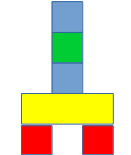
\includegraphics[width=0.25\textwidth]{figs/Chapter4/BlockGoal.png}
       \label{subfig:goal}
   }\hfill
    %~
	\subfigure[Un possible état de départ (vue de haut).)]{
        \centering
        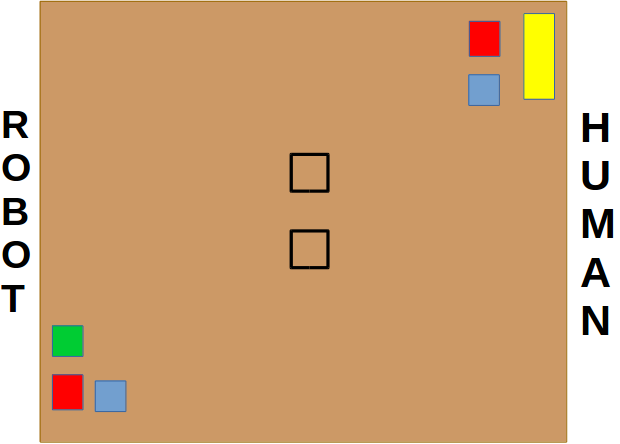
\includegraphics[width=0.4\textwidth]{figs/Chapter4/SetUp.png}
       \label{subfig:setUp}
   }
    \caption{Description de la tâche de construction de blocs. L'Homme et le robot doivent construire une pile ensemble.}
    \label{fig:blocksBuildingTask}
\end{figure*}

Pour illustrer les bénéfices de ce travail, nous avons utilisé une tâche inspirée de celle présentée dans \cite{clodic2014key}. Un Homme et un robot doivent réaliser une construction avec des blocs colorés comme représenté Fig.~\ref{subfig:goal}. Au début de la tâche, l'Homme et le robot ont chacun plusieurs blocs de couleur à leur disposition comme par exemple Fig. \ref{subfig:setUp}. Deux emplacements identiques sont placés au centre de la table pour indiquer ou mettre les deux premiers cubes rouges.

\begin{figure*}[!h]
\centering
	\subfigure[Plan initial.]{
        \centering
        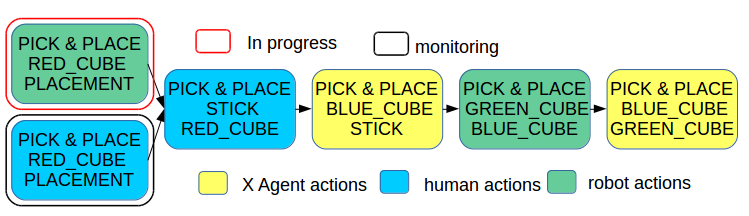
\includegraphics[width=0.7\textwidth]{figs/Chapter4/second_plan.png}
       \label{subfig:initPlan}
   }
    %~
	\subfigure[Le robot choisit de mettre son cube rouge sur l'emplacement à sa droite.]{
        \centering
        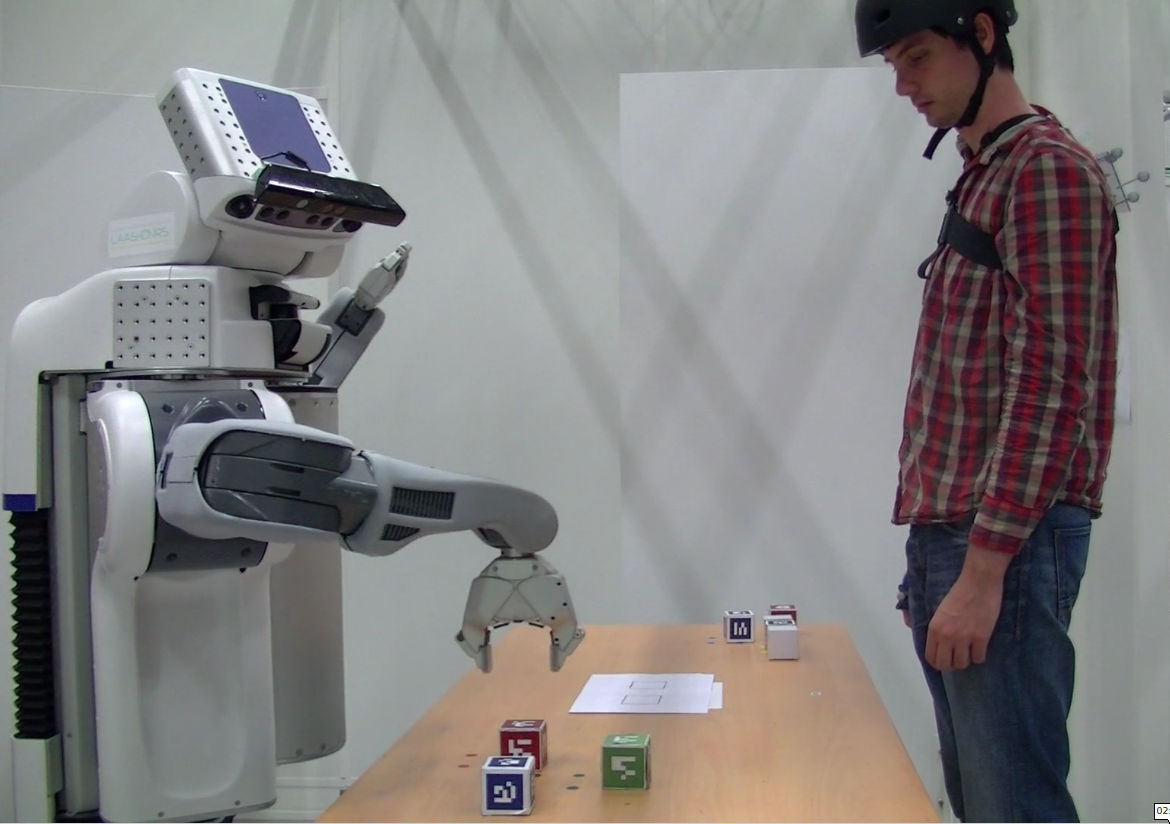
\includegraphics[width=0.4\textwidth]{figs/Chapter4/screen_shot1.jpeg}
       \label{subfig:redCube}
   }\hfill
    %~
	\subfigure[L'Homme pose son cube sur l'emplacement que le robot a choisit.]{
        \centering
        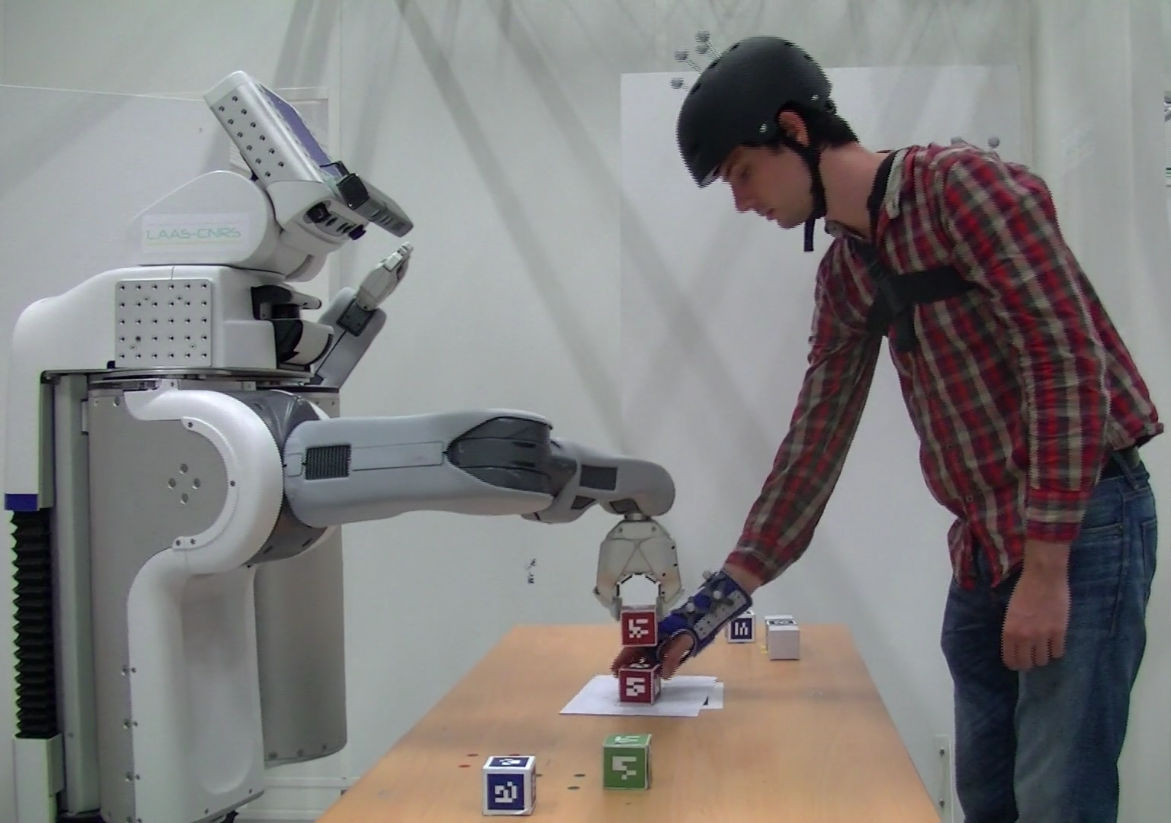
\includegraphics[width=0.4\textwidth]{figs/Chapter4/screen_shot2.jpeg}
       \label{subfig:humanPlace}
   }
    %~
	\subfigure[Le robot s'adapte en changeant son choix d'emplacement.]{
        \centering
        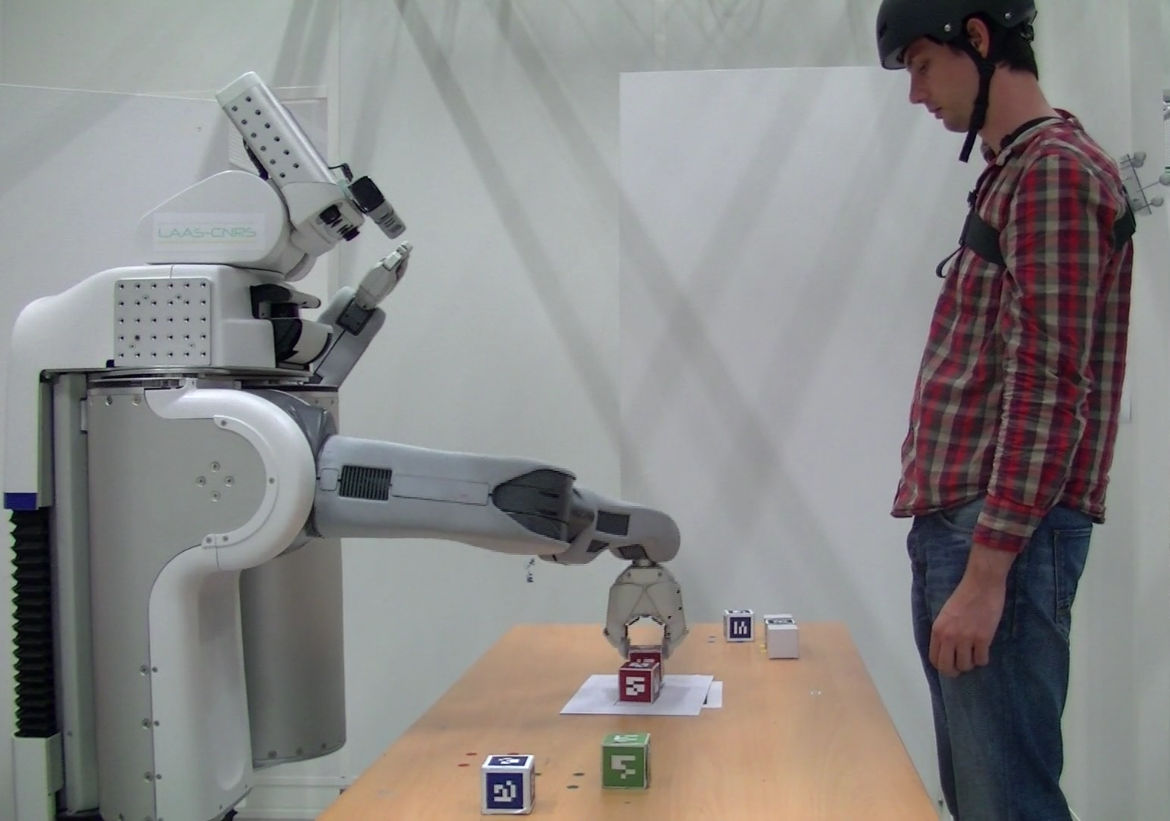
\includegraphics[width=0.4\textwidth]{figs/Chapter4/screen_shot3.jpeg}
       \label{subfig:robotAdapts}
   }\hfill
    %~
	\subfigure[Deuxième plan.]{
        \centering
        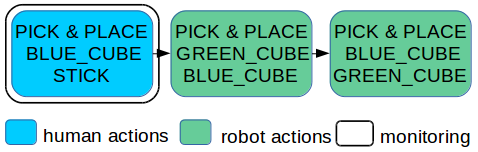
\includegraphics[width=0.4\textwidth]{figs/Chapter4/third_plan.png}
       \label{subfig:thirdPlan}
   }
    \caption{Exemple illustratif d'une tâche de construction de blocs.}
\end{figure*}

Le plan produit initialement par HATP pour réaliser la tâche peut être trouvé Fig.~\ref{subfig:initPlan}. Le robot attrape le cube rouge à sa disposition et choisit de le placer sur l'emplacement à sa droite (Fig. \ref{subfig:redCube}). Cependant, l'Homme prend son cube rouge et choisit de le placer sur le même emplacement que celui choisi par le robot (Fig.~\ref{subfig:humanPlace}). Le robot interrompt son action et s'adapte en plaçant son cube sur l'autre emplacement (Fig.~\ref{subfig:robotAdapts}). L'homme pose alors le bâton jaune sur les cubes rouges. Dans cet exemple, le robot utilise le mode \textbf{négociation} pour choisir qui va mettre le premier cube bleu. Le robot demande donc à l'Homme si il veut poser le cube bleu ("Voulez-vous poser le cube bleu ?"). L'Homme répond oui, le robot calcule donc un nouveau plan ou il posera le second cube bleu Fig.~\ref{subfig:thirdPlan}. Finalement, l'Homme et le robot effectuent leurs dernières actions et réalisent la tâche avec succès.

\newpage
\subsection{Évaluation du système}

\subsubsection{Tâche et conditions}

Afin d'évaluer le nouveau système développé concernant la gestion des plans partagés par le robot, nous avons développé une tâche d'inventaire. Dans cette tâche, l'Homme et le robot doivent scanner différents cubes de couleur et les ranger dans une boîte de même couleur. Au début de la tâche chaque agent a une pile de cubes de différentes couleurs à laquelle seulement lui peut accéder. Ces piles contiennent des cubes bleus, verts et rouges. Pour que les cubes soit scannés, les agents doivent les poser un par un sur une des deux zones de scan sur la table devant le robot (voir Fig.~\ref{fig:setUpSimu}). Une fois un cube sur une zone, le robot peut le scanner en orientant sa tête vers le cube et en allumant une lumière rouge en direction du cube (voir Fig.~\ref{fig:scan}). Une fois un cube scanné, il peut être rangé dans une boite de la même couleur. Le robot a accès à une boite bleue et à une boite rouge tandis que l'Homme a accès à une boite verte et à une boite rouge (voir Fig.~\ref{fig:setUpSimu}). Cette tâche comporte deux particularités intéressantes pour notre système:
\begin{itemize}
\item Comme la pile de l'homme et ses boîtes sont situées dans des pièces différentes que celle du robot (voir Fig.~\ref{fig:setUpSimu}), si le robot scanne un cube quand l'Homme est parti chercher ou ranger un cube, l'Homme ne pourra pas savoir que le cube a été scanné sauf si le robot l'en informe (pas d'effets visibles).
\item La répartition des boites entre les agents fait que seul le robot peut ranger les cubes bleus, seul l'Homme peut ranger les cubes verts mais qu'ils peuvent tous les deux ranger les cubes rouges.
\end{itemize}

\begin{figure}[!h]
	\centering
    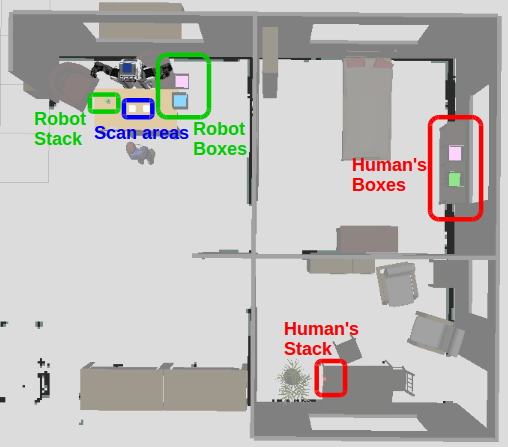
\includegraphics[width=0.9\textwidth]{figs/Chapter5/SetUpSimu.png}
    \caption{Etat initial pour la tâche d'inventaire. L'Homme et le robot doivent prendre les cubes de leur pile pour les mettre sur une zone de scan. Puis, le robot doit scanner le cube et enfin chaque cube doit être rangé dans une boite de même couleur. L'Homme a accès à une boite verte et à une boite rouge tandis que le robot a accès à une boite bleue et à une boite rouge.}
    \label{fig:setUpSimu}
\end{figure}

Nous avons évalué notre système en simulation et lors d'une étude utilisateur. Pour faire cela, nous avons comparé 4 différentes conditions :
\begin{itemize}
\item avec le système original, appelé \textbf{système de référence (RS)}, où toutes les décisions du robot sont prises durant l'élaboration du plan et sans estimation des états mentaux de l'Homme:
\begin{itemize}
\item \textbf{RS-NONE mode :} le robot ne verbalise rien (sauf en cas de stricte nécessité).
\item \textbf{RS-ALL mode :} le robot informe à propos de toutes les actions qu'il doit faire et que l'homme doit réaliser ainsi qu'à propos de toutes les actions manquées par l'Homme.
\end{itemize}
\item avec le nouveau système développé présenté précédemment (\textbf{NS}) :
\begin{itemize}
\item \textbf{NS-N mode :} le robot utilise le mode \textbf{négociation} pour prendre une décision concernant les actions de \textit{l'agent X}.
\item \textbf{NS-A mode :} le robot utilise le mode \textbf{adaptation} pour prendre une décision concernant les actions de \textit{l'agent X}.
\end{itemize}
\end{itemize}

\subsubsection{Évaluation en simulation}

Pour évaluer notre système en simulation, nous avons fait tourner la tâche avec différents états de départ ou les piles des agents étaient aléatoirement composées. Durant ces simulations, le robot était confronté à plusieurs types d'Hommes simulés :
\begin{itemize}
\item \textit{l'Homme "aimable" (cas \textbf{K}) :} qui adapte son comportement à ce que verbalise le robot. Concernant les cubes rouges, il peut choisir de ne jamais les ranger (\textbf{lazy-K}), les ranger systématiquement (\textbf{hurry-K}) ou les ranger avec une probabilité de 50\% (\textbf{50\%-K})
\item \textit{l'Homme "têtu" (cas \textbf{S}) :} qui n'adapte pas son comportement à ce que verbalise le robot. Concernant les cubes rouges, il peut choisir de ne jamais les ranger (\textbf{lazy-S}), les ranger systématiquement (\textbf{hurry-S}) ou les ranger avec une probabilité de 50\% (\textbf{50\%-S})
\end{itemize}
Dans tous les cas, l'Homme participe activement au dépôt des cubes de sa pile sur les zones de scan et au rangement des cubes verts et répond aux questions posées par le robot.

Les données mesurées durant ces simulations sont :
\begin{itemize}
\item \textit{le nombre d'interactions verbales :} entre l'Homme et le robot (information donnée par le robot ou question posée), Tab.~\ref{tab:verbalInteraction}.
\item \textit{le nombre de décisions incompatibles :} les deux acteurs prennent la même décision concernant une action (les deux essayent de la réaliser ou de ne pas la réaliser), Tab.~\ref{tab:incompatibleDecisions}.
\item \textit{le temps d'exécution total :} pour réaliser la tâche, Fig.~\ref{fig:resTime}.
\end{itemize}

\begin{table*}[!h]
\centering
  \begin{tabular}{|c||c|c|c|c|}
  \hline
     & \textbf{RS-NONE} & \textbf{RS-ALL} & \textbf{NS-N} & \textbf{NS-A} \\
  \hline
  \hline
     \textbf{50\%-K} & 2.4 (0.84) & 20.7 (1.34) & 3.4 (1.51) & 2 (1.33) \\
  \hline
     \textbf{hurry-K} & 1.8 (0.79) & 21.1 (2.08) & 1.9 (1.10) & 2.2 (1.13) \\
  \hline
     \textbf{lazy-K} & 3.0 (1.33) & 21 (1.56) & 3.3 (1.42) & 1.6 (1.17) \\
  \hline
     \textbf{50\%-S} & 2.5 (1.43) & 23.9 (1.59) & 3.3 (1.49) & 1.7 (0.95)\\
  \hline
     \textbf{hurry-S} & 1.5 (0.97) & 20.9 (1.29) & 2.4 (1.89) & 1.9 (0.99)\\
  \hline
     \textbf{lazy-S} & 3.2 (0.92) & 25.2 (1.55) & 2.8 (1.68) & 1.8 (1.14)\\
  \hline
  \end{tabular}
   \caption{\textbf{Nombre d'interactions verbales} : questions posées par le robot dans le mode négociation et nombre d'informations verbalisées. Ces résultats correspondent à la moyenne sur 10 essais et leur déviation standard associée.}
   \label{tab:verbalInteraction}
\end{table*}

Plusieurs choses peuvent être observées par rapport aux résultats obtenus :
\begin{itemize}
\item le mode \textbf{RS-NONE} est celui comportant le plus de décisions incompatibles (du fait que le robot ne communique et de s'adapte pas par rapport aux cubes rouges et aux choix des zones de scan). Ce mode comporte également les plus grands temps d'exécution, plus spécialement dans le cas de l'Homme "têtu" car le robot perd du temps à attendre qu'il exécute des actions qu'il ne veut pas réaliser ou à attendre que l'Homme range un cube dont il ne sait pas qu'il a été scanné.
\item comme attendu, le mode \textbf{RS-ALL} est celui avec le plus d'interactions verbales. Cependant, ces interactions verbales ne suffisent pas à supprimer toutes les décisions incompatibles, surtout dans le cas de l'homme "têtu" ou le temps d'exécution est également plus élevé.
\item on peut voir que les performances du \textbf{nouveau système} sont globalement meilleures que celles de l'ancien système. En effet pour beaucoup moins d'informations verbalisées, il permet de supprimer les décisions incompatibles et de réduire le temps d'exécution dans le cas de l'Homme "têtu". Le mode \textbf{adaptation} obtient les mêmes résultats que le mode \textbf{négociation} mais avec moins d'interactions verbales.
\end{itemize}


\begin{table*}[!h]
\centering
  \begin{tabular}{|c||c|c|c|c|}
  \hline
     & \textbf{RS-NONE} & \textbf{RS-ALL} & \textbf{NS-N} & \textbf{NS-A} \\
  \hline
  \hline
     \textbf{50\%-K} & 2.9 (0.99) & 0.9 (0.57) & 0.6 (0.7) & 0.3 (0.48) \\
  \hline
     \textbf{hurry-K} & 2.5 (0.97) & 1.0 (0.94) & 0.6 (0.52) & 0.4 (0.52)\\
  \hline
     \textbf{lazy-K} & 3.5 (1.08) & 0.8 (0.63) & 0.5 (0.7) & 0.5 (0.53) \\
  \hline
     \textbf{50\%-S} & 2.9 (1.45) & 1.9 (0.99) & 0.6 (0.52) & 0.5 (0.97) \\
  \hline
     \textbf{hurry-S} & 2.3 (1.34) & 1.0 (0.82) & 0.5 (0.53) & 0.4 (0.52) \\
  \hline
     \textbf{lazy-S} & 3.5 (0.97) & 2.6 (1.84) & 0.3 (0.67) & 0.4 (0.52)  \\
  \hline
  \end{tabular}
   \caption{\textbf{Nombre de décisions incompatibles} : les deux acteurs prennent la même décision concernant une action (les deux essayent de la réaliser ou de ne pas la réaliser). Ces résultats correspondent à la moyenne sur 10 essais et leur déviation standard associée.}
   \label{tab:incompatibleDecisions} 
\end{table*}

\begin{figure}[!h]
	\centering
    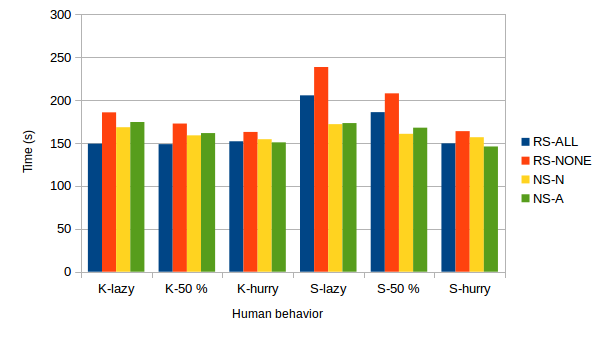
\includegraphics[width=0.9\textwidth]{figs/Chapter5/Time.png}    \caption{Temps en secondes nécessité pour chaque système pour réaliser la tâche dans chaque condition (moyennes sur 10 essais).}
    \label{fig:resTime}
\end{figure}

\subsubsection{Étude utilisateur}

\begin{figure}[!t]
	\centering
    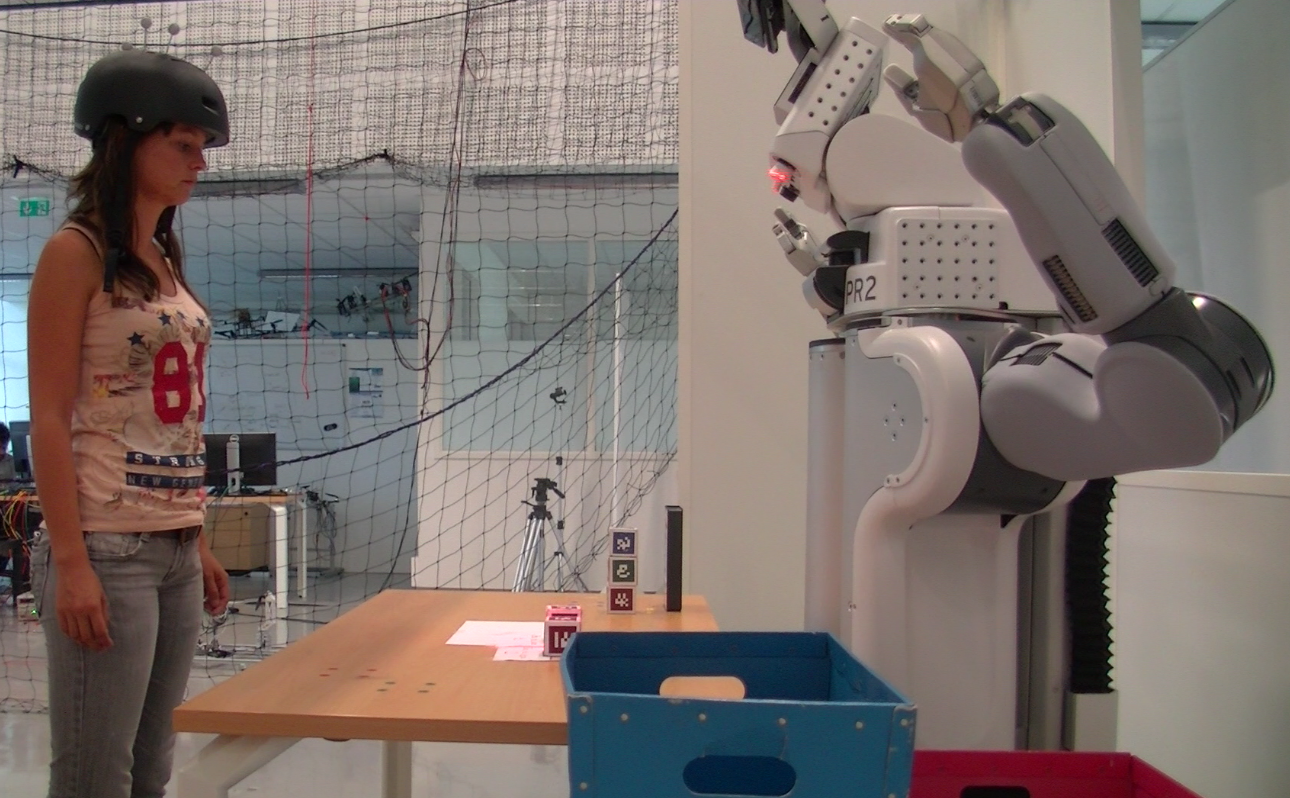
\includegraphics[width=0.7\textwidth]{figs/Chapter5/Scan.png}
    \caption{Le robot PR2 interagissant avec un sujet pour réaliser la tâche. Le robot scanne un objet avant de le ranger.}
    \label{fig:scan}
\end{figure}


\paragraph{Adaptation de la tâche pour l'étude utilisateur:}

Avant de réaliser l'étude utilisateur, nous avons effectué quelques pré-tests qui nous ont permis d'identifier plusieurs problèmes et d'y remédier avec des adaptations de la tâche :
\begin{itemize}
\item \textbf{introduction d'une cassette rouge :} afin d'assurer qu'il y ait forcement une prise de décision par rapport à un objet rouge (de temps en temps la configuration faisait qu'aucune décision n'était nécessaire), nous avons ajouté une cassette rouge qui doit être scannée et rangée une fois que tous les cubes ont été rangés. L'Homme et le robot ont chacun initialement une cassette rouge mais une seule doit être scannée et rangée.
\item \textbf{Tâche de distraction :} afin d'être surs d'obtenir un manque de connaissance à un moment de la tâche (de temps en temps l'homme ne s'absentait jamais lors d'une action de scan), nous avons rajouté une tâche de construction avec des Légos pour le sujet à un moment de la tâche dans un lieu ou il ne peut pas voir le robot.
\end{itemize}


\paragraph{Questionnaire et protocole:}

21 sujets (8 femmes et 13 hommes) ont interagi avec le robot pour réaliser la tâche dans les quatre conditions décrites précédemment. L'ordre de ces conditions et les compositions des piles des agents étaient aléatoires.
A leur arrivée, les participants étaient introduits à l'environnement de travail et au robot par l’expérimentateur. Ensuite, les participants avaient à lire les consignes de la tâche et l’expérimentateur vérifiait leur bonne compréhension. Les participants réalisaient une rapide tâche de familiarisation avant de réaliser la vraie tâche.
Après chaque interaction avec le robot (pour chaque condition), les participants avaient à remplir un questionnaire leur permettant d'évaluer le comportement du robot. Comme nous n'avons pas trouvé dans la littérature existante de questionnaires permettant d'évaluer la prise de décision haut niveau d'un robot lors d'une tâche de collaboration avec l'Homme, nous avons conçu ce questionnaire en nous basant sur le modèle d'expérience utilisateur UX \cite{mahlke2008user} et en ajoutant des dimensions spécifiques à la prise de décision. Ce questionnaire est composé de plusieurs dimensions :
\begin{itemize}
\item \textbf{Dimension de collaboration}, basée sur \cite{weistroffer2014etude} et permettant d'évaluer la perception de l'utilité et de l'utilisabilité du robot \cite{davis1989perceived}.
\item \textbf{Dimension d'interaction}, basée sur \cite{lallemand2015creation} et permettant d'évaluer l'intention d'utilisation \cite{davis1989perceived}.
\item \textbf{Dimension de perception du robot}, basée sur le questionnaire Godspeed \cite{bartneck2009measurement} et permettant d'évaluer comment le sujet perçoit le robot en général \cite{hassenzahl2003thing}.
\item \textbf{Dimension émotions,} reprise de l'AffectButton \cite{broekens2013affectbutton} et permettant d'évaluer les émotions du sujet lors de l'interaction.
\item \textbf{Dimension verbale} permettant d'évaluer comment le sujet a perçu les interactions verbales avec le robot.
\item \textbf{Dimension d'action} permettant d'évaluer comment le sujet a perçu la prise de décision du robot par rapport au choix d’exécution des actions.
\end{itemize}
Ces dimensions étaient évaluées grâce à des questions où le sujet devait se placer sur une échelle de 100, sauf pour la dimension émotion ou le sujet avait à choisir entre plusieurs smileys.

\paragraph{Hypothèses:} 
Nous avons émis plusieurs hypothèses avant l'étude :
\begin{itemize}
\item \textbf{Hypothèse 1 :} le nouveau système sera préféré par les utilisateurs à l'ancien système.
\item \textbf{Hypothèse 2 :} concernant le nouveau système, au contraire des résultats de simulation, le mode négociation sera préféré par les utilisateurs au mode adaptation.
\end{itemize}

\paragraph{Résultats:}

La cohérence interne de questionnaire a été vérifiée à la suite de cette étude (alpha de Cronbach supérieur à 0,7 pour toutes les dimensions du questionnaire). Concernant les scores des différentes conditions, les résultats totaux du questionnaire peuvent être trouvés en Fig~\ref{fig:resUSTotal}.

\begin{figure}[!h]
	\centering
    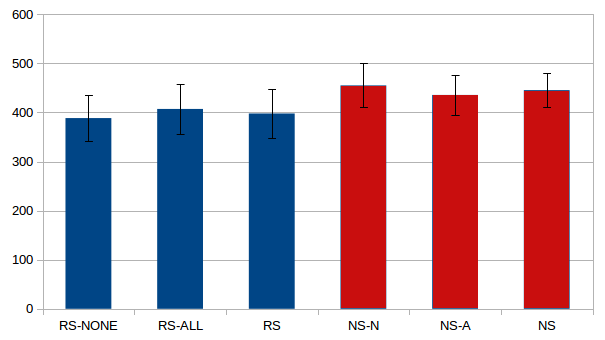
\includegraphics[width=0.7\textwidth]{figs/Chapter5/Total.png}
    \caption{Scores totaux du questionnaire utilisateur. Addition des scores de toutes les dimensions précédemment remis sur une échelle de 100.}
    \label{fig:resUSTotal}
\end{figure}

Les scores du nouveau système (NS) ont été trouvés significativement plus élevés (p < 0.05) que ceux de l'ancien système (RS). Cela permet donc de vérifier la première hypothèse comme quoi le nouveau système a été préféré des sujets. Concernant le nouveau système, si l'on regarde la dimension verbale du questionnaire, le score de la condition \textbf{négociation} a été trouvé significativement plus élevé que celui de la condition \textbf{adaptation} (p < 0.05). Il n'y a pas eu de différence significative concernant les autres dimensions. Comme la seule différence entre ces deux modes consiste à poser ou non une question quand il y avait une décision à prendre concernant un objet rouge (comportement verbal), nous pouvons donc considérer la seconde hypothèse comme validée également.

\subsubsection{Conclusion}

L'évaluation du système en simulation et lors d'une étude utilisateur a permis de montrer que le nouveau système développé a de meilleures performances et une meilleure appréciation par l'utilisateur que l'ancien système. Concernant les deux modes possible du nouveau système, des utilisateurs naïfs comme ceux de l'étude utilisateur préfère le mode \textbf{négociation}. Cependant, pour des utilisateurs plus experts, le mode \textbf{adaptation} a montré de meilleurs résultats en simulation. L'étude utilisateur nous a également permis de développer et valider un questionnaire permettant d'évaluer la prise de décision haut niveau du robot lors d'une tâche de collaboration avec l'Homme. 


\newpage
\section{Autres contributions à l'action conjointe Homme-Robot}

\subsection{Communication non-verbale: qu'est ce que le robot doit faire avec sa tête ?}

\subsubsection{Motivations et précédents travaux}

Pour communiquer entre eux quant ils collaborent sans être trop verbeux, les hommes utilisent fréquemment la communication non-verbale \cite{ekman1969repertoire, depaulo1992nonverbal}. Durant l'action conjointe Homme-Robot, le robot doit également être capable de communiquer à son partenaire toutes les informations dont il a besoin sans être trop intrusif. Pour cela, il doit donc être capable d'avoir un comportement non-verbal adapté à l'action conjointe. La communication non-verbale vient de multiples sources (expression faciales \cite{labarre1947cultural}, postures \cite{mehrabian1969significance}, regard \cite{mutlu2009designing}, etc...). Dans cette thèse, nous nous sommes concentré sur l'utilisation de la tête du robot, remplaçant les signaux donnés par le regard en l'absence de pupilles pour le robot \cite{imai2002robot}.

Les sciences sociales ont permis de déterminer plusieurs utilisations du regard durant l'action conjointe entre Hommes :
\begin{itemize}
\item \textbf{Aide au dialogue et à la prise de tour :} le regard est très utilisé lors du dialogue \cite{argyle1976gaze} et plus spécifiquement pour signaler les changements d'orateur \cite{kendon1967some}. 
\item \textbf{Aide à la compréhension des actions :} les acteurs d'une action conjointe vont agir différemment que lorsqu'ils agissent seul \cite{becchio2010toward, vesper2010minimal}. Plus spécifiquement, l'utilisation du regard lors d'une action va permettre aux partenaires de mieux interpréter les intentions de l'acteur \cite{castiello2003understanding, pierno2006gaze}.
\item \textbf{Aide à la compréhension des états mentaux :} l'observation du regard du partenaire permet de mieux prendre sa perspective afin de mieux estimer ses connaissances \cite{furlanetto2013through}.
\end{itemize}

En robotique, plusieurs études ont montré l’intérêt du comportement non-verbal du robot \cite{furlanetto2013through, haring2012studies}. Beaucoup de travaux se sont concentrés sur l'utilisation de la tête lors du dialogue \cite{mutlu2009footing, boucher2010facilitative, skantze2014turn}. Seuls quelques uns portent sur l'utilisation du regard durant l'action conjointe et ont montré qu'un bon comportement de la part du robot aide à la coordination lors de l'exécution du plan partagé \cite{lallee2013cooperative} et à la prise de décision de l'Homme \cite{boucher2012reach}.

\subsubsection{Réflexion concernant les signaux et comportements nécessaires}

Sur la base d'une étude bibliographique des comportements humains et des travaux sur la tête du robot, nous avons identifié ce que nous pensons être des composants nécessaires à un bon comportement de la tête du robot lors de l'action conjointe :
\begin{itemize}
\item \textbf{Lorsque le robot agit :} lors de ses actions, le robot doit utiliser sa tête à la fois pour la bonne réalisation de l'action d'un point de vue fonctionnel (présence de caméras à l'intérieur de la tête) mais également pour indiquer à ses partenaires ce qu'il fait et ce qu'il va faire ensuite. 
\item \textbf{Lorsque le robot parle :} lors d'un dialogue, il est important pour le robot de regarder l'homme au bon moment ainsi que les objets dont il parle.
\item \textbf{Le robot observe :} le robot doit se servir de sa tête pour montrer son intérêt et sa compréhension des actions de l'Homme.
\item \textbf{Le robot se coordonne :} le robot doit fournir les signaux appropriés et nécessaires au bon déroulement du plan partagé.
\end{itemize}

\subsubsection{Étude approfondie de certains signaux }

Nous avons étudié dans plus de détails certains composants des comportements définis précédemment. Pour faire cela, nous avons mené une étude utilisateur en ligne à base de vidéos. Dans cette étude, nous avons demandé à 59 personnes (30 femmes et 29 hommes) de regarder plusieurs vidéos courtes ou le comportement de la tête du robot changeait et d'évaluer ces comportements grâce à un petit questionnaire. Dans ces vidéos, l'Homme et le robot avaient à construire une pile de cubes colorés (comme illustré Fig.~\ref{fig:videoTask}).

\begin{figure*}[!t]
\centering
	\subfigure[Début de la tâche. Le cube bleu et le cube vert sont accessibles par l'Homme et les cubes noir et rouge sont accessibles par le robot.]{
        \centering
        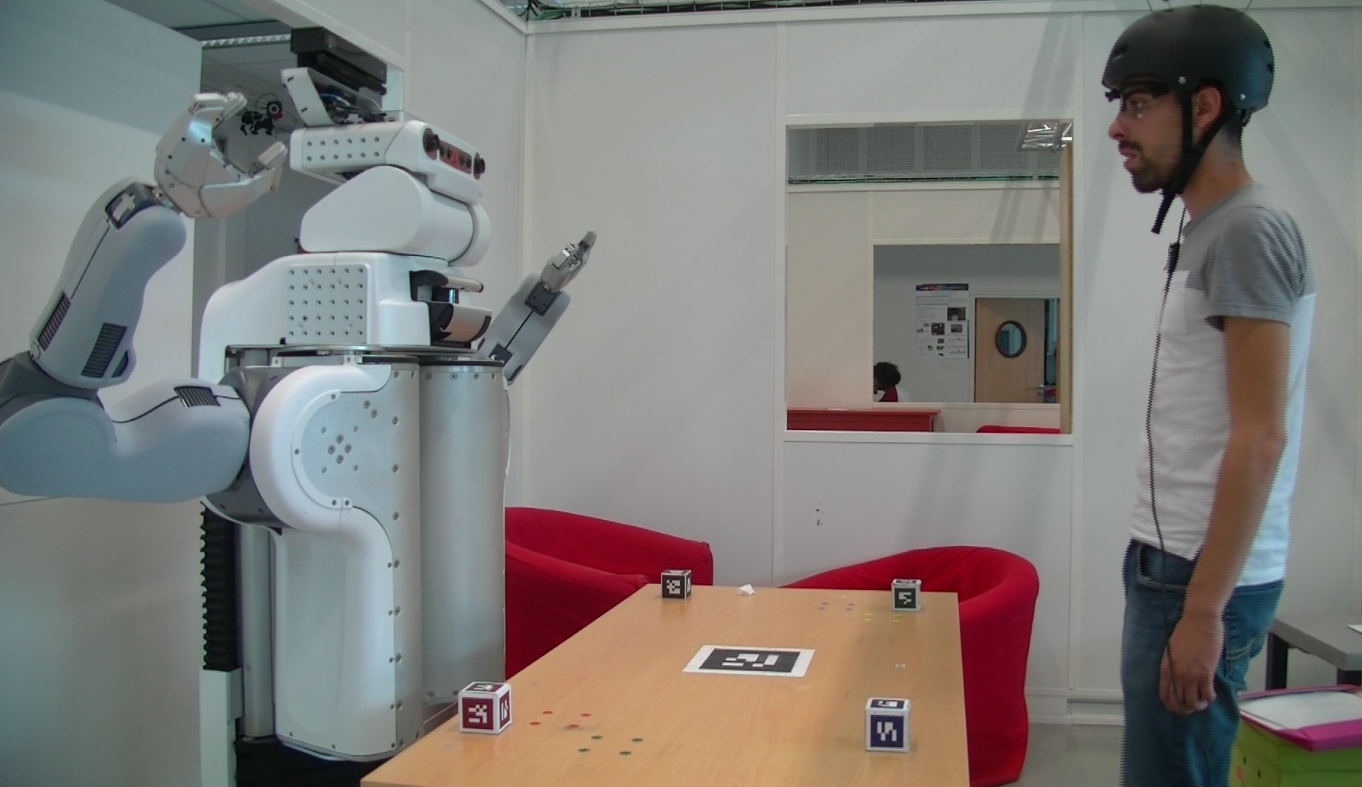
\includegraphics[width=0.45\textwidth]{figs/Chapter6/VideoInit.png}
       \label{subfig:videoInit}
   }\hfill
    %~
	\subfigure[Fin de la tâche. La pile doit être construite dans un ordre précis (rouge, noir, bleu, vert).]{
        \centering
        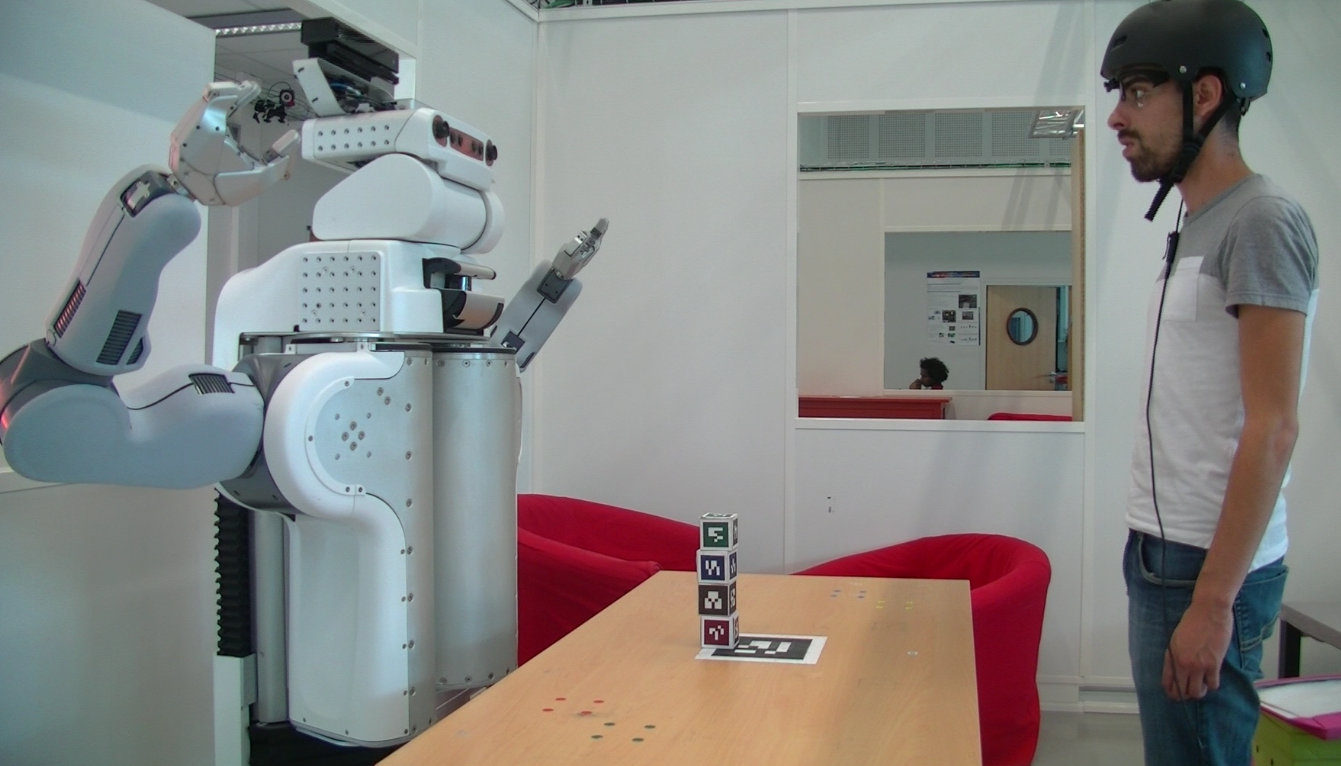
\includegraphics[width=0.45\textwidth]{figs/Chapter6/VideoGoal.png}
       \label{subfig:videoGoal}
   }
    \caption{Tâche utilisée dans l'étude utilisateur en ligne. Dans cette tâche, l'Homme et le robot doivent construire une pile de cubes colorés.}
    \label{fig:videoTask}
\end{figure*}

Les comportements testés et les résultats obtenus sont les suivants :
\begin{itemize}
\item \textbf{Anticipation des actions du robot :} nous avons comparé un comportement du robot ou il anticipait sa prochaine action avec sa tête (il regarde le cube à prendre avant de commencer son action) au même comportement sans cette anticipation. Nous n'avons pas trouvé de différence significative entre ces deux comportements. En effet, certains des sujets étaient perturbés par le fait que le robot regarde le cube avant d'agir et d'autres n'ont pas vu la différence. Une possible explication pour cela est que la tâche ne demandait pas d'anticipation de la part du robot car les deux participants savaient quelle action était nécessaire à chaque moment (ordre de la pile prédéfini).
\item \textbf{Suivre l'activité de l'homme :} nous avons comparé différents moyens pour le robot de suivre avec sa tête l'activité de l'Homme. Dans la première condition, le robot regardait la main de l'homme dès qu'elle était en mouvement et la tête sinon. Dans la seconde, le robot regardait la main de l'Homme quand elle était dans une zone de travail définie au dessus de la table et la tête sinon. Finalement, dans la dernière condition, le robot regardait la main de l'Homme quand elle était en mouvement et dans la zone de travail et la tête sinon. Cette dernière condition a été significativement préférée aux deux autres par les sujets.
\item \textbf{Montrer la compréhension des actions de l'Homme :} nous avons comparé un comportement ou le robot marquait un arrêt avec sa tête quand l'Homme réalisait une action de manière à montrer qu'il avait détecté l'action à une condition sans cet arrêt. Nous n'avons pas trouvé de différence significative entre ces deux conditions, les sujets ayant du mal à trouver les différences entre les deux vidéos.
\item \textbf{Gérer l'inaction de l'Homme :} dans ces vidéos, l'Homme mettait du temps à réaliser une de ses actions. Nous avons comparé trois différentes réaction de la part du robot. Dans la première, le robot ne changeait pas son comportement de base face à cette inaction. Dans la seconde, le robot donnait un signal à l'Homme avec sa tête en regardant le cube que l'Homme devait prendre. Dans la dernière, le robot donnait un signal similaire mais cette fois ci regardait le cube de l'Homme puis la pile. Les deux conditions ou le robot donnait un signal à l'Homme ont été notées significativement mieux que celle sans signal montrant l'importance du signal du robot. Aucune différence n'a été trouvée entre les deux différents signaux.
\item \textbf{Aide à la prise de tour :} nous avons comparé différentes manières pour le robot de gérer le changement d'acteur dans la tâche (passage d'une action du robot à une action de l'Homme). Dans deux conditions, le robot ne donnait pas de signal particulier à l'Homme. Il regardait simplement l'Homme soit à la fin de son action dans une condition, soit après s'être retiré de son action dans l'autre condition. Dans les deux autres conditions, le robot regardait le cube que l'Homme devait poser avant de regarder l'Homme. Comme pour les deux précédentes conditions, le robot faisait cela à la fin de son action dans une condition et après s'être retiré dans l'autre condition. Les deux conditions où le robot regardait le cube de l'Homme ont été trouvées significativement meilleures que les deux autres, montrant l’intérêt du signal du robot. Aucune différence n'a été trouvée concernant le timing du signal (avant ou après le retrait).
\item \textbf{Choisir un objet d'attention :} dans le dernier scénario, l'Homme commençait à prendre un cube pendant que le robot était toujours en train de poser le sien. Dans une condition, le robot continuait son action sans regarder l'Homme. Dans la seconde condition, le robot regardait l'Homme mais sans interrompre sa propre action. Dans la dernière condition, le robot interrompait son action pour regarder celle de l'Homme. La condition ou le robot ne regarde pas l'Homme a été trouvée significativement moins bonne que les deux autres. Aucune différence n'a été trouvée entre les deux autres conditions. Cela montre l'importance pour le robot de regarder l'action de l'Homme même si il doit pour cela interrompre sa propre action.
\end{itemize}

\subsubsection{Proposition d'architecture pour le comportement de la tête du robot}

A partir de l'étude bibliographique et des résultats de l'étude présentée précédemment, nous avons proposé une architecture pour gérer la tête du robot. Cette architecture peut être trouvée Fig.~\ref{fig:headArchi}.

\begin{figure}[!h]
	\centering
    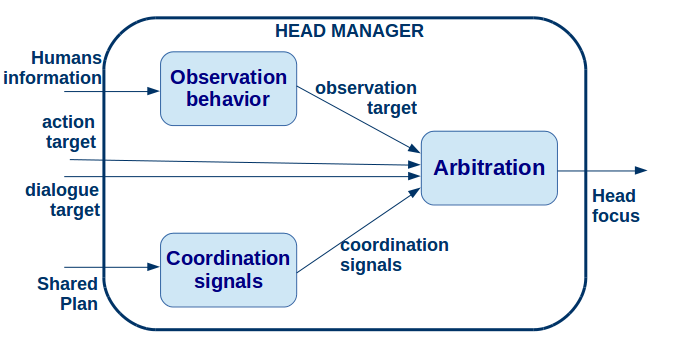
\includegraphics[width=0.9\textwidth]{figs/Chapter6/Head_archi.png}
    \caption{Architecture pour gérer la tête du robot. Un module d'arbitrage choisit où le robot doit regarder en se basant sur plusieurs comportements et signaux produits par des modules en amont.}
    \label{fig:headArchi}
\end{figure}

Un premier module permet au robot de générer un comportement pour montrer sa compréhension de l'activité de l'Homme. Basé sur les résultats de l'étude précédente, nous proposons d'implémenter un comportement où le robot regarde successivement la tête et la main de l'Homme en se basant sur le mouvement de la main et sa position (dans ou en dehors de zones de travail). Nous proposons également d'implémenter un comportement qui permet au robot de répondre aux regards de l'Homme (le robot regarde l'Homme si il le regarde et regarde l'objet de l'attention de l'Homme si l'Homme regarde fixement un objet).

En entrée de l'architecture proposée, nous trouvons des points d’intérêt venant du module d’exécution d'action du robot et du module de dialogue. Ces deux modules fournissent tous les deux l'objet ou la personne la plus pertinente à regarder en fonction de l'action du robot et de la conversation en cours.

Un autre module permet de créer des signaux à donner à l'Homme concernant l'exécution du plan partagé. Nous proposons d'implémenter les deux signaux étudiés précédemment (signal quand l'Homme n'agit pas et signal d'aide à la prise de tour). 

Finalement, un module d'arbitrage permet de choisir entre les différents comportements et signaux générés par les autres modules en se basant sur ce que fait le robot et les différentes priorités des signaux et comportements.

\newpage
\subsection{Combiner apprentissage et planification}

\subsubsection{Motivations et travaux précédents}

Concernant la prise de décision en robotique, on retrouve deux grandes écoles de pensée qui ont chacune leurs avantages et désavantages : l'apprentissage et les processus déterministes (ou planification). L'apprentissage est généralement "peu coûteux" au sens où une décision est prise rapidement et une solution va toujours être proposée quelque soit le problème. Cependant, la phase d'apprentissage requière une grande quantité de données et/ou une longue période d'apprentissage durant laquelle le robot va produire des comportements inconsistants et perturbants pour l'utilisateur humain. La planification va être plus lente à prendre une décision, particulièrement dans le cas d'un environnement ou d'une tâche complexe, mais va pouvoir prendre en compte des règles sociales et assurer la validité de la solution proposée dans son ensemble. L'idée de ce travail est de combiner ces deux techniques dans le contexte de le prise de décision pour l’interaction Homme-Robot.

Ces deux écoles de pensées sont inspirées des différents comportements des mammifères et de l'Homme : le comportement \textit{dirigé vers un but} pour la planification et le comportement \textit{habituel} pour l'apprentissage \cite{dickinson1985actions}. Différentes études ont été menées en neuroscience pour trouver comment alterner entre ces comportements \cite{pezzulo2013mixed, lesaint2014modelling, viejo2015modeling}. En robotique, de nombreux travaux ont été réalisés en planification \cite{ingrand2014deliberation} et en apprentissage \cite{kober2011learning, martins2010learning, stulp2013robot} mais peu d'entre eux se concentrent sur comment combiner ces approches.


\subsubsection{Présentations des différents experts}

\begin{figure}[!h]
	\centering
    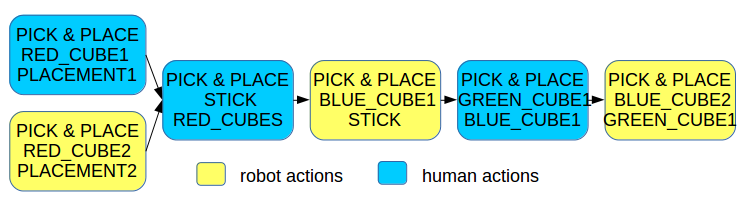
\includegraphics[width=0.9\textwidth]{figs/Chapter7/SharedPlan.png}
    \caption{Un exemple de plan produit par HATP. Ce plan permet à un Homme et à un robot de nettoyer une table en enlevant tous les objets dessus, la nettoyant puis replaçant tous les objets enlevés précédemment.}
    \label{fig:examplePlan}
\end{figure}

Dans le travail présenté dans cette thèse, deux experts ont été utilisés pour modéliser les deux comportements évoqués précédemment :
\begin{itemize}
\item Le comportement \textit{dirigé vers un but} est fourni par HATP \cite{Lallement2014hatp}, un planificateur HTN conçu pour le contexte de l'interaction Homme-robot. HATP prend en compte les préconditions et effets des différentes actions possibles pour construire un plan qui permet d'atteindre un but précis depuis un contexte donné (e.g. Fig.~\ref{fig:examplePlan}). HATP permet de calculer un plan complet qui permet d'atteindre un but donné et qui prend en compte des coûts concernant l'Homme. Cependant, il ne permettra pas d'apprendre du comportement de l'Homme en direct, les coûts étant codés à l'avance. Son temps de décision sera plus lent que celui de l'autre expert mais ne nécessite pas de période d'apprentissage.
\item Le comportement \textit{habituel} est produit par un algorithme d'apprentissage par renforcement sans modèle \cite{renaudo2014design} qui permet d'apprendre une action à exécuter pour chaque état possible en se basant sur un principe de récompense. Cet algorithme est implémenté comme un réseau neuronal (voir Fig.~\ref{fig:Qlearning}). Cet algorithme permet de toujours proposer rapidement une action à exécuter par le robot. Cependant une longue phase d'apprentissage est nécessaire pendant laquelle le robot aura un comportement inconsistant au début et à chaque changement de la tâche.
\end{itemize}

\begin{figure}[!h]
	\centering
    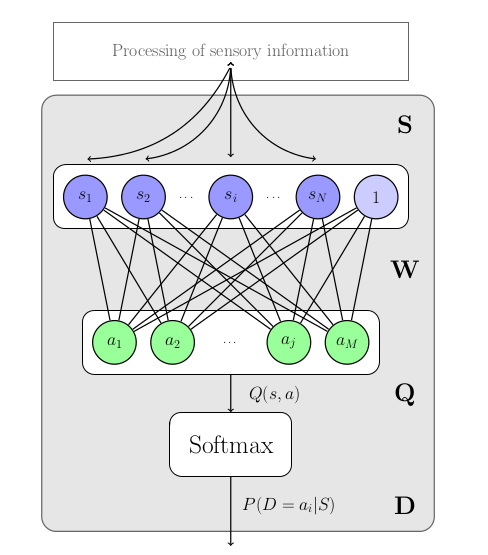
\includegraphics[width=0.6\textwidth]{figs/Chapter7/Qlearning.png}
    \caption{L'expert du comportement habituel est un algorithme d'apprentissage implémenté comme un réseau neuronal. Il reçoit en entrée un état $S$ qui est projeté sur un neurone d'entrée $s_i$ définissant une activité d'entrée. L'activité est propagée grâce aux poids du réseau neuronal $W$ pour générer une activité sur le niveau d'action. Cette activité correspond à la valeur $Q(S, a_j)$ et est convertie en une probabilité de distribution permettant à l'expert de prendre une décision $D$ sur la prochaine action à exécuter.}
    \label{fig:Qlearning}
\end{figure}



\subsubsection{Première architecture : une preuve de concept}


\paragraph{Architecture :}

La première architecture développée pour combiner les deux experts peut être trouvée Fig.~\ref{fig:FirstArchi}. Dans cette architecture les deux experts sont placés en parallèle. Le module d'évaluation de la situation prend les données de la perception et maintient l'état du monde courant. Cet état du monde est utilisé par la supervision pour calculer la récompense et par les experts pour prendre une décision. Les propositions des deux experts sont envoyées au méta-contrôleur qui décide de l'action à exécuter (de manière aléatoire). Le superviseur exécute l'action avec l'aide des modules de plus bas niveau.

\begin{figure}[!h]
	\centering
    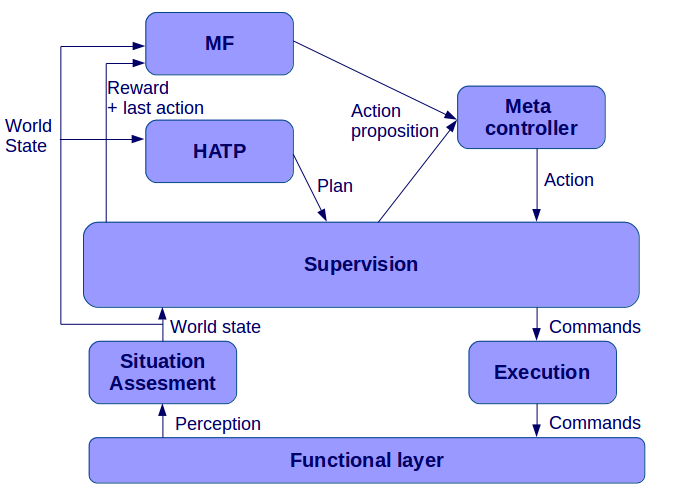
\includegraphics[width=0.8\textwidth]{figs/Chapter7/FirstArchi.png}
    \caption{Première architecture développée pour combiner les deux experts.}
    \label{fig:FirstArchi}
\end{figure}


\paragraph{Tâche :}

Nous avons testé cette architecture sur une tâche simple en simulation illustrée Fig.~\ref{fig:firstTask}. Dans cette tâche, l'Homme et le robot doivent enlever des objets d'une table et les mettre dans une boite rose. Au début de l’interaction, deux objets sont accessibles uniquement par le robot et un autre uniquement par l'Homme. La boite est accessible uniquement par le robot. Pour réaliser la tâche, l'Homme et le robot peuvent exécuter différentes actions (prendre un objet, ranger un objet, s'échanger un objet ou attendre).

Le comportement de l'Homme est simulé dans cette expérience. L'Homme est collaboratif : il exécute toutes les actions prévues pour lui dans HATP et participe à tous les échanges d'objets entrepris par le robot.

\begin{figure*}[!h]
\centering
	\subfigure[Situation initiale]{
        \centering
        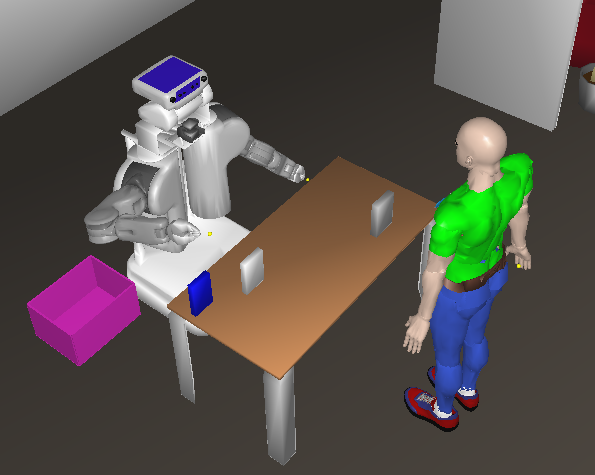
\includegraphics[width=0.45\textwidth]{figs/Chapter7/initFirstTask.png}
       \label{subfig:initFirst}
   }\hfill
    %~
	\subfigure[Situation finale]{
        \centering
        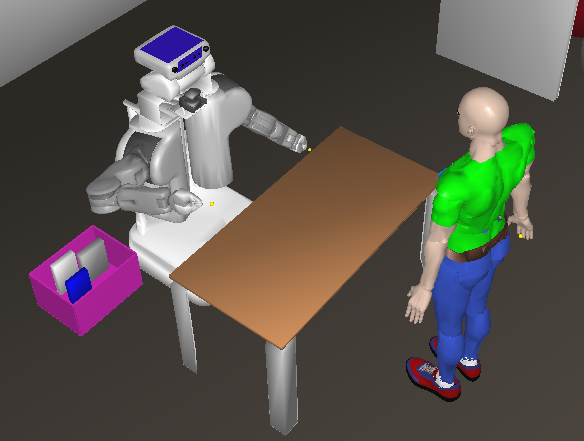
\includegraphics[width=0.47\textwidth]{figs/Chapter7/endFirstTask.png}
       \label{subfig:endFirst}
   }
    \caption{Tâche utilisée pour tester la première architecture. L'Homme et le robot doivent enlever les objets de la table et les mettre dans la boite rose.}
    \label{fig:firstTask}
\end{figure*}


\paragraph{Résultats :}

Pour tester notre architecture, nous avons réalisé la tâche avec chaque expert seul dans un premier temps puis avec la combinaison des deux. La tâche a été réalisée en boucle dans un temps imparti. Le critère principal utilisé ici pour évaluer le système est le nombre de fois qu'il est capable de réaliser la tâche dans ce temps imparti. Les résultats pour 10 simulations de 30 minutes dans chaque condition peuvent être trouvés Fig.~\ref{subfig:rewardsFirstTask}. On peut observer une faible performance du MF seul (algorithme d'apprentissage) due à son manque de connaissances initial. La combinaison des deux experts a de bien meilleures performances bien qu'elles restent en dessous de celles d'HATP seul. En effet, la tâche étant simple à résoudre pour HATP, son plan est toujours optimal. Finalement, nous pouvons voir Fig.~\ref{subfig:weightsFirstTask} que la combinaison du MF et d'HATP permet au MF d'apprendre bien plus vite que quand il est seul.

\begin{figure*}[!h]
\centering
	\subfigure[Moyenne des récompense obtenues sur 10 simulations de 30 minutes (une récompense par tâche achevée).]{
        \centering
        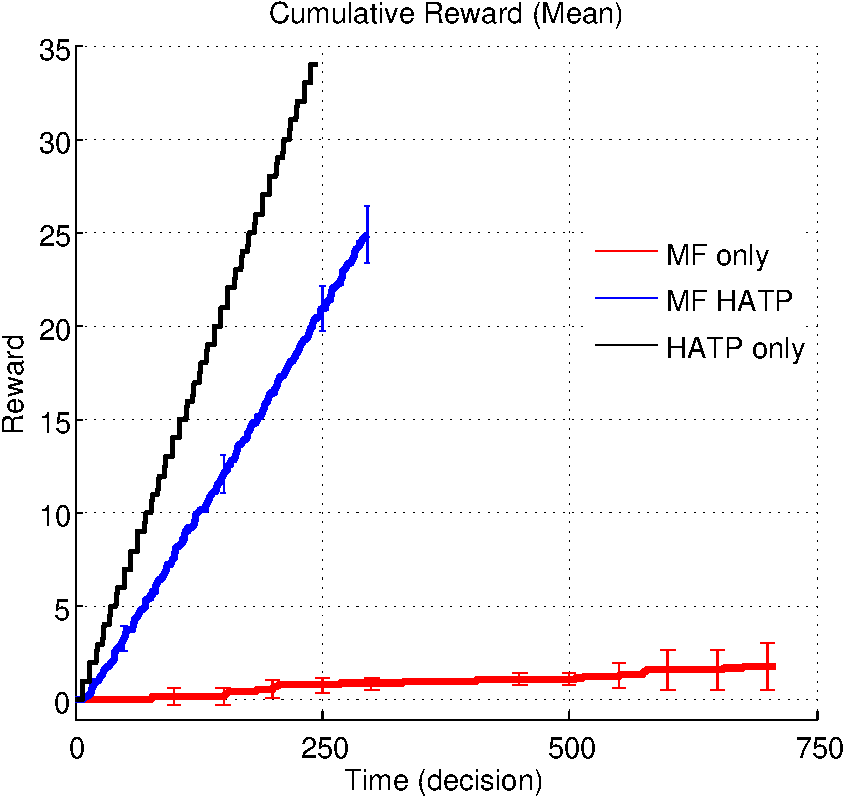
\includegraphics[width=0.45\textwidth]{figs/Chapter7/rewardsFirstTask.pdf}
       \label{subfig:rewardsFirstTask}
   }\hfill
    %~
	\subfigure[Moyenne de l'évolution des poids de connexion du MF seul et avec HATP. Plus l'amplitude est élevée et plus le MF a appris qu'elle action exécuter.]{
        \centering
        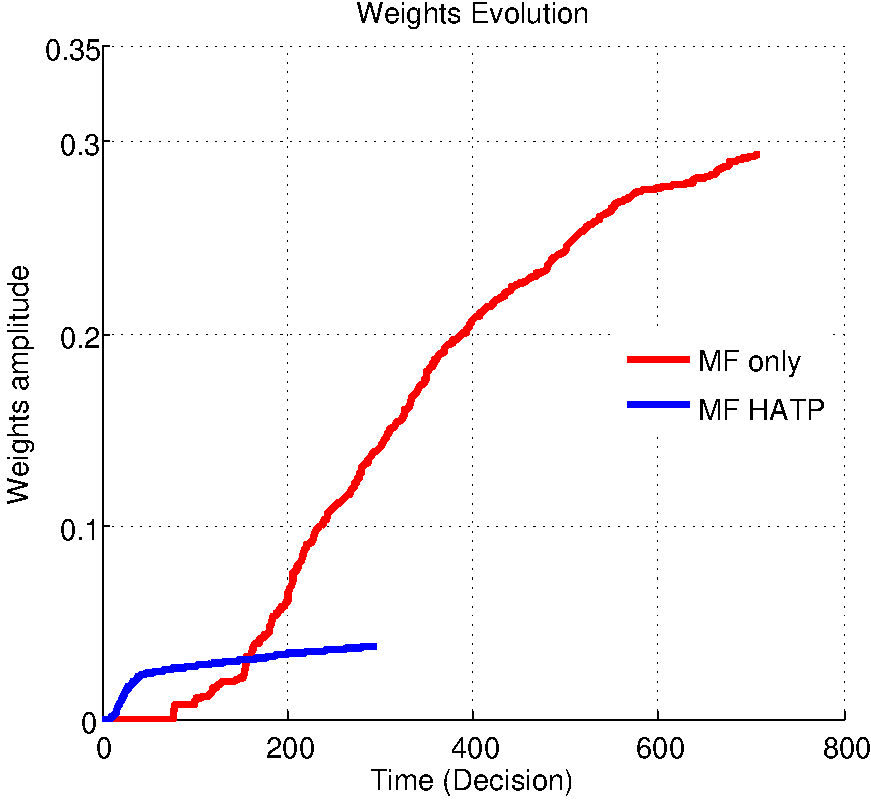
\includegraphics[width=0.45\textwidth]{figs/Chapter7/WeightEvolFirstTask.pdf}
       \label{subfig:weightsFirstTask}
   }
    \caption{Performances de l'architecture testée comparées aux experts seuls.}
    \label{fig:resultsFirstTask}
\end{figure*}

Les premiers résultats obtenus montrent que la combinaison d'HATP et du MF permet d’accélérer l'apprentissage du MF. Cependant, la tâche étant très simple, HATP n'a pas de difficulté quand il décide seul. 

\subsubsection{Seconde architecture: les limitations}

Dans un second temps, nous avons amélioré l'architecture et l'avons testée sur une tâche plus complexe afin de démontrer l’intérêt du système.

\paragraph{Architecture :}

Comme l'un des principaux avantages du MF par rapport à HATP est son temps de calcul, nous avons modifié l'architecture comme représenté Fig.~\ref{fig:SecondArchi}. Dans cette version de l'architecture le meta-contrôleur est en amont des experts. Un expert ne sera activé uniquement que lorsque le meta-contrôleur choisira qu'il doit décider de la prochaine action. 

\begin{figure}[!h]
	\centering
    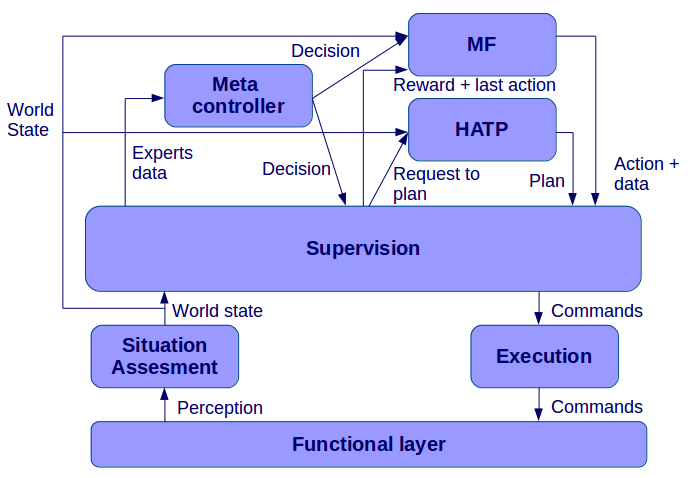
\includegraphics[width=0.8\textwidth]{figs/Chapter7/SecondArchi.png}
    \caption{Seconde architecture développée pour combiner les deux experts.}
    \label{fig:SecondArchi}
\end{figure}

Nous avons également introduit dans cette nouvelle architecture un nouveau critère pour la prise de décision du meta-contrôleur (précédemment aléatoire). Ce critère est basé sur le coût de chaque expert (temps à trouver une solution) et son erreur de prédiction. 

\paragraph{Tâche :}

Pour augmenter la complexité de la tâche, nous avons dans un premier temps augmenté sa combinatoire. Dans la nouvelle tâche il y a maintenant 6 objets qui doivent aller dans deux boites différentes en fonction de leur couleur. Ces objets sont initialement placés de manière aléatoire sur 7 emplacements possibles sur la table au début de la tâche comme Fig.~\ref{fig:SecondArchi}. De nouvelles actions sont également possibles pour le robot, il peut maintenant replacer un objet sur un des emplacements ou naviguer à une autre position près de la table.

\begin{figure}[!h]
	\centering
    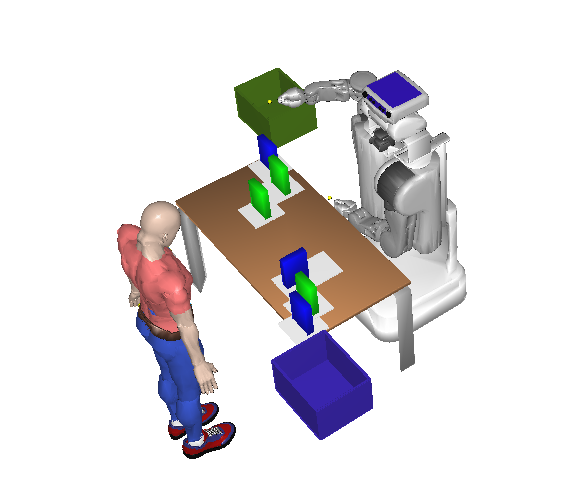
\includegraphics[width=0.8\textwidth]{figs/Chapter7/InitSecondScenario1.png}
    \caption{Tâche utilisée pour tester la seconde architecture. L'Homme et le robot doivent enlever les objets de la table et les mettre dans les boites de même couleur.}
    \label{fig:SecondArchi}
\end{figure}

Nous avons également ajouté dans la tâche des difficultés géométriques qui ne peuvent pas être gérées par la planification (certains objets supposés accessibles ne peuvent en fait pas être attrapés par le robot). Finalement, nous avons également implémenté différents comportements pour l'homme simulé (plus ou moins coopératifs).

\paragraph{Résultats :}

Comme la tâche est plus complexe, nous avons légèrement augmenté le temps de simulation. Comme précédemment, nous avons testé le système avec chaque expert séparément puis avec la combinaison des deux. Logiquement, HATP présente de meilleurs résultats avec un Homme plus collaboratif et le MF présente de pauvres résultats seul. Cependant, nous n'avons pas réussi à avoir des résultats pour la combinaison des deux experts supérieurs à ceux d'HATP seul. Cela est dû au fait qu'avec une tâche plus complexe, l'effet d'accélération d'HATP sur l'apprentissage du MF n'est plus suffisant pour lui permettre d'apprendre une solution pour la tâche et donc lui permettre d'aider le système. 

Afin d'obtenir un système plus performant, de possibles améliorations seraient de retravailler l'algorithme d'apprentissage afin de mieux l'adapter au contexte et lui permettre d'apprendre plus rapidement. Une autre amélioration possible serait de chercher un nouveau critère d'arbitrage pour le meta-contrôleur. Enfin, il serait intéressant de permettre à HATP d'obtenir un retour de ce qu'apprend le MF afin d'adapter en ligne ses modèles de planification.


\begin{figure*}[!h]
\centering
	\subfigure[Moyenne des récompenses obtenues sur 10 simulations de 40 minutes pour HATP seul (une récompense par tâche achevée).]{
        \centering
        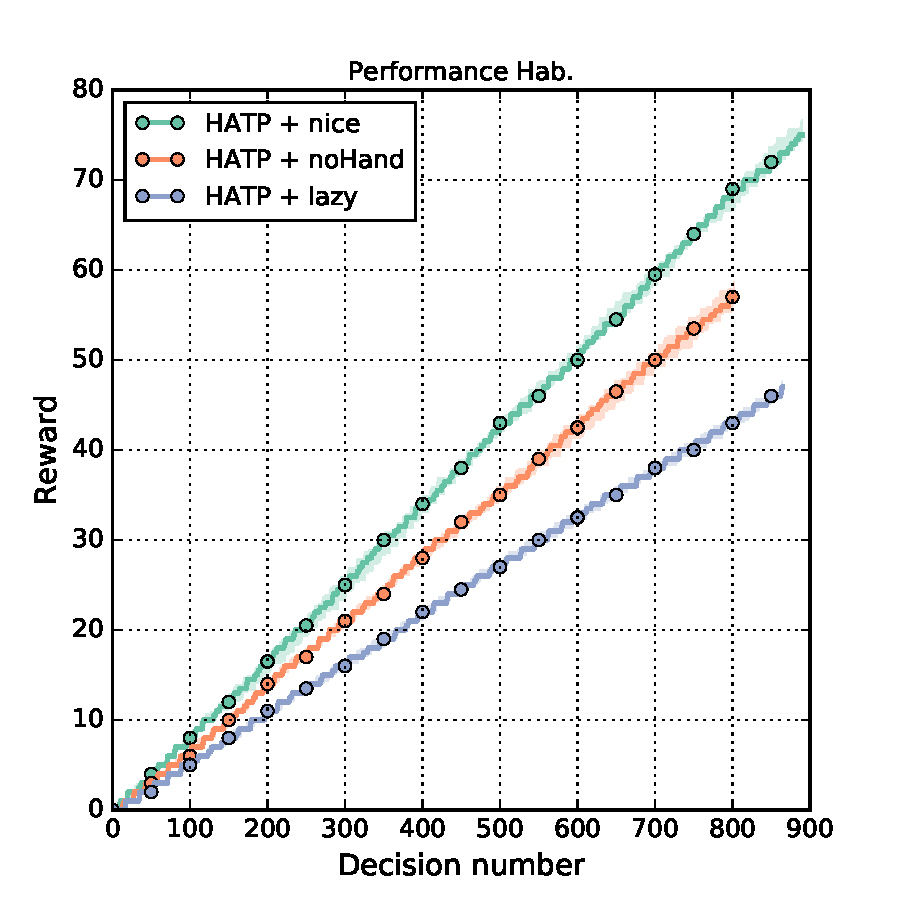
\includegraphics[width=0.45\textwidth]{figs/Chapter7/reward_HATP.pdf}
       \label{subfig:reward_HATP}
   }\hfill
    %~
	\subfigure[Moyenne des récompenses obtenues sur 10 simulations de 40 minutes pour le MF seul (une récompense par tâche achevée).]{
        \centering
        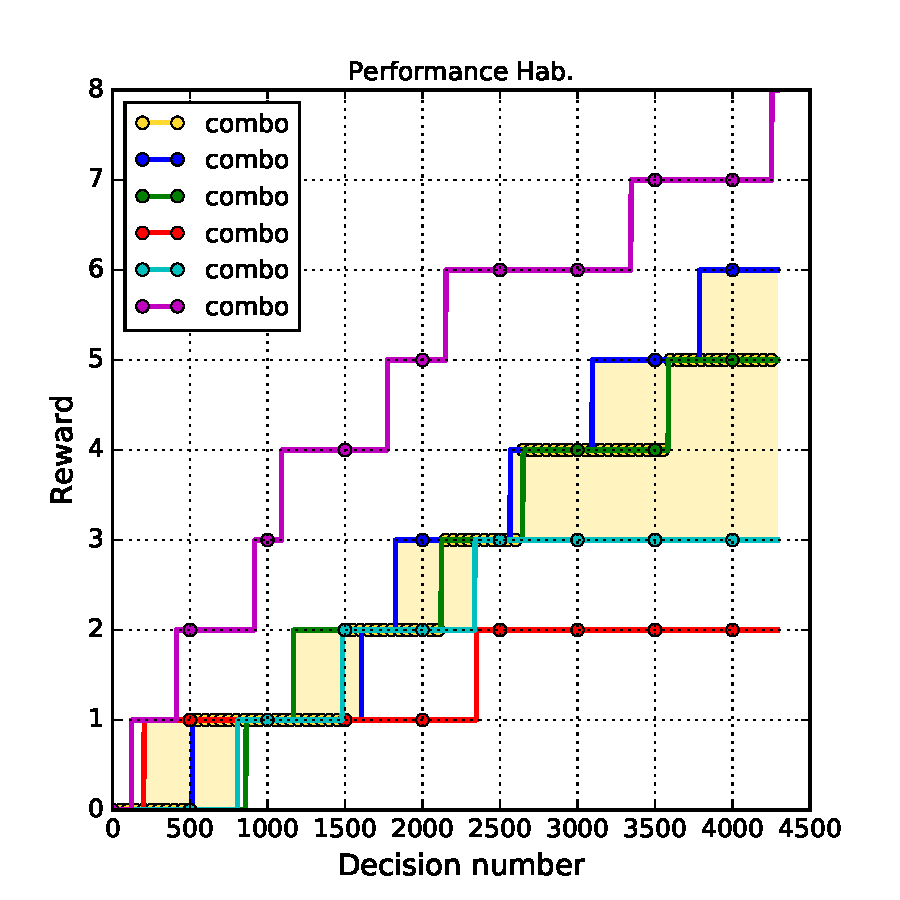
\includegraphics[width=0.45\textwidth]{figs/Chapter7/reward_MFalone.pdf}
       \label{subfig:reward_MFalone}
   }
    %~
	\subfigure[Moyenne des récompenses obtenues sur 10 simulations de 40 minutes pour la combinaison des deux experts (une récompense par tâche achevée).]{
        \centering
        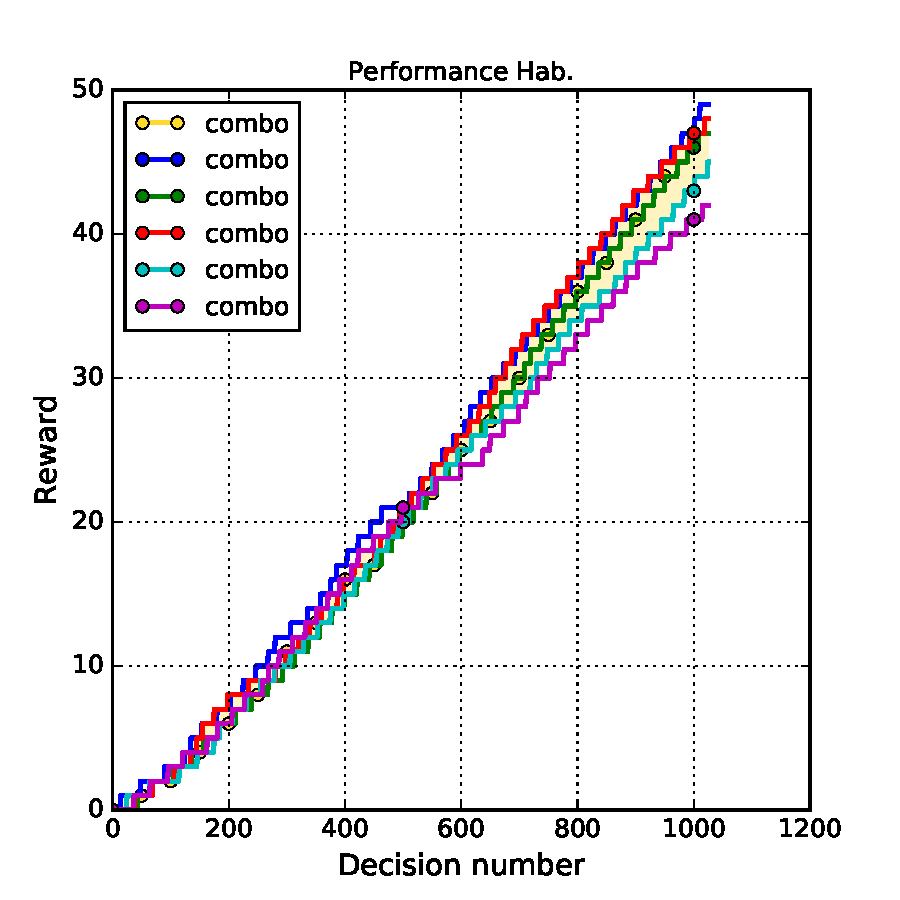
\includegraphics[width=0.45\textwidth]{figs/Chapter7/reward_combo.pdf}
       \label{subfig:reward_combo}
   }
    \caption{Moyenne des récompenses obtenues dans chaque condition.}
    \label{fig:resultsFirstTask}
\end{figure*}

\newpage
\section{Conclusion}

Plusieurs contributions sont présentées dans ce manuscrit :
\begin{itemize}
\item Dans un premier temps, nous avons étudié les bases de l'action conjointe entre Hommes et comment ces principes s'appliquent à l'interaction Homme-robot afin de construire un superviseur pour la décision lors de l'action conjointe Homme-robot. 
\item Dans un second temps nous avons étudié comment améliorer la gestion des plans partagés par le robot. Nous avons d'abord étendu l'estimation des états mentaux de l'Homme par le robot au plan partagé, puis, nous avons amélioré les algorithmes de gestion du plan pour rendre le comportement du robot plus flexible. Enfin, nous avons évalué ces deux contributions en simulation et en conditions réelles grâce à une étude utilisateur.
\item Enfin, nous avons présenté deux autres contributions à l'interaction Homme-Robot. La première concerne la gestion de la tête du robot lors d'une tâche collaborative. La seconde cherche à combiner deux méthodes de prise de décision par le robot : la planification et l'apprentissage.
\end{itemize}

\selectlanguage{english}

\ifdefined\included
\else
\bibliographystyle{StyleThese}
\bibliography{These}
\end{document}
\fi
